% Main document of the project, this will include all the other parts involving the documentation...

\documentclass[a4paper]{article}
\usepackage[utf8]{inputenc}
\usepackage[T1]{fontenc}

%% Sets page size and margins
\usepackage[a4paper,top=3cm,bottom=2cm,left=3cm,right=3cm,marginparwidth=1.75cm]{geometry}

%% Useful packages
\usepackage[table,xcdraw]{xcolor}
\usepackage{longtable}
\usepackage{amsmath}
\usepackage{floatrow}
\usepackage{graphicx}
\graphicspath{ {./images/} }
\usepackage[colorinlistoftodos]{todonotes}
\usepackage[colorlinks=true, allcolors=blue]{hyperref}
\usepackage{amsmath}
\usepackage{chngcntr}
\usepackage{wrapfig}
\usepackage{eurosym}
\usepackage{caption}
\usepackage{subcaption}
\usepackage{listings}
\usepackage{placeins}
\usepackage{multicol}
\usepackage{verbatim}
\usepackage{csvsimple}
\usepackage{listings}
\usepackage[spanish]{babel}
\renewcommand\spanishtablename{Tabla}
\selectlanguage{spanish}
\usepackage{colortbl}
\usepackage{cite}
\usepackage{xr}

\usepackage[toc,page]{appendix}
\usepackage{pdflscape}

\expandafter\def\expandafter\appendixpagename%
\expandafter{\expandafter\Huge\appendixpagename}

\usepackage{afterpage}

\addto\captionsspanish{%
  \renewcommand\appendixname{\Huge Apéndices}
  \renewcommand\appendixpagename{\Huge Apéndices}
}

\captionsetup[table]{position=bottom}

\renewcommand{\lstlistingname}{Código}% 
\renewcommand{\lstlistlistingname}{Lista de código}% List of Listings -> List of Algorithms

% extracted from internet: https://timmurphy.org/2014/01/27/displaying-code-in-latex-documents/
\definecolor{lbcolor}{rgb}{0.93,0.93,0.93}
\lstset{  
    frame=tb, % draw a frame at the top and bottom of the code block
    tabsize=4, % tab space width
    showstringspaces=false, % don't mark spaces in strings
    numbers=left, % display line numbers on the left
    commentstyle=\color{green}, % comment color
    keywordstyle=\color{blue}, % keyword color
    stringstyle=\color{red},
    backgroundcolor=\color{lbcolor}
}

\definecolor{main-color}{rgb}{0.6627, 0.7176, 0.7764}
\definecolor{back-color}{rgb}{0.1686, 0.1686, 0.1686}
\definecolor{string-color}{rgb}{0.3333, 0.5254, 0.345}
\definecolor{key-color}{rgb}{0.8, 0.47, 0.196}
\lstdefinestyle{idlstyle}
{
    language = C++,
    keywordstyle = {\color{key-color}},
    keywordstyle = [3]{\color{blue}},
    otherkeywords = {in, int ,interface, out, inout},
    morekeywords = [3]{in, out, inout}
}

\setcounter{secnumdepth}{3}
\setcounter{tocdepth}{3}

% \title{Integrating COMPSs and OmpSs Programming Models to support distributed heterogeneous computing environments}
\title{Integrating COMPSs and OmpSs Programming Models to support distributed heterogeneous computing environments}
\author
{
Marc Domínguez de la Rocha
\and
Rosa M. Badia
\and
Jorge Ejarque
}

\date{Abril 2019}

\begin{document}

\maketitle

\newpage
\renewcommand{\contentsname}{Índice}
\tableofcontents
\newpage

%GEP

\chapter{Introducción}

\section{Contexto}

Hoy en día se tiende a tener distintos recursos de cómputo en un solo dispositivo, por ejemplo, en un teléfono móvil ya tenemos al menos un procesador y una tarjeta gráfica, pero no tan sólo en el ámbito más cotidiano (aunque no nos demos cuenta), sino que en los más profesionales y especializados está siendo también cada vez más común la heterogeneidad de los recursos de computación en servidores, \textit{clusters} y supercomputadores. 

\par\bigskip

Programar estos dispositivos, que cuentan con esta heterogeneidad no es una tarea sencilla, un procesador no se programa de la misma manera que un acelerador, ni dos aceleradores tienen por qué programarse de la misma manera, existen una gran variedad de modelos de programación que nos brindan estas facilidades pero esta gran variedad se torna abrumadora y a veces repercute en la portabilidad de las aplicaciones. Es por esto que nos hemos decidido a hacer este proyecto, para mejorar en la medida de lo posible la facilidad de desarrollo y portabilidad de una aplicación en estas plataformas cada vez más complejas.

\par\bigskip

Si se facilita a la comunidad este tipo de programación, no solo habría una disminución del esfuerzo a realizar por parte del programador (hasta ahora, abismal), si no que mejoraría el desempeño de las aplicaciones que utilizasen todos los recursos que hay a su disposición en una máquina. Esto motiva la realización del proyecto, que pretende facilitar la gestión de estos recursos de computación en entornos distribuidos, brindando un método robusto y eficiente para programar aplicaciones en estos entornos.

\par\bigskip

Este proyecto es un Trabajo de Fin de Grado del Grado en Ingeniería Informática, especializado en el área de Ingeniería de Computadores. El grado es impartido por la \textit{Facultat d'Informàtica de Barcelona (FIB)} centro perteneciente a la \textit{Universitat Politècnica de Catalunya (UPC)}. 
\par\bigskip

El proyecto se ha desarrollado conjuntamente con el \textit{Barcelona Supercomputing Center (BSC)}, hemos estudiado como integrar los modelos de programación \textit{COMPSs} y \textit{OmpSs} para alcanzar este objetivo, se ha implementado y evaluado un prototipo.
%Indagar en cuales son estas caracteristicas? 

\subsection{Actores}

Los actores en este proyecto son las personas que tomen parte en él, ya sea de manera directa o indirecta. Con esto quiero decir, que tanto las personas que han tomado parte en el desarrollo \textit{per se} como las personas que se nutran de este, son los actores.

\begin{itemize}
 \item \textbf{Desarrollador:} La figura del desarrollador \textbf{es} la persona que ha trabajado de manera más directa en el proyecto. En este proyecto únicamente hay un desarrollador que ha elaborado la documentación que leerás a continuación y ha dado forma a los objetivos tangibles del proyecto.  
 \item \textbf{Director y codirector:} Pese a que el desarrollador ha tenido el papel principal en el proyecto, el director y el codirector han guiado a este en el camino abierto que es el desarrollo del proyecto. Periódicamente ha habido reuniones de seguimiento donde se han supervisado las actividades del proyecto y su correcta realización.
 \item \textbf{Barcelona Supercomputing Center:} De manera directa el centro otorga al desarrollador un lugar de trabajo y un equipo informático. Por otra parte, cuenta con el soporte por parte de los equipos de desarrollo de \textit{COMPSs} (del cual forma parte el desarrollador) y de \textit{OmpSs} para cualquier incidencia relacionada con su \textit{software} y derivados.
 \item \textbf{Beneficiarios:} El proyecto facilita el desarrollo de aplicaciones paralelas en entornos heterogéneos distribuidos, de manera que se espera que los beneficiarios sean cualquier desarrollador de esta, sea de la organización que sea.
\end{itemize}

\section{Estado del arte}

Existen muchos modelos de programación, véanse \textit{OpenMP}\cite{dagum1998openmp}, \textit{OmpSs}\cite{duran2011ompss}, \textit{MPI}\cite{walker1996mpi}, \textit{COMPSs}\cite{badia2015comp} y un largo etcétera. De alguna manera el objetivo en común fue y es aprovechar los cada vez más abundantes recursos en las máquinas, que finalmente no sólo han crecido en abundancia si no en diversidad. La filosofía sigue siendo la misma, sacar el mayor rendimiento posible a nuestras máquinas. 
\par\bigskip

Para esto son necesarios modelos de programación que nos den la posibilidad de utilizar los recursos y nos ayuden a explotar la posible sinergia entre estos en ciertas aplicaciones. 
\par\bigskip

La diferencia más elemental entre los modelos, es en como se gestiona la memoria, o más bien cómo se estructura en el modelo.

\begin{itemize}
\item \textbf{Memoria compartida:} En un modelo con memoria compartida como \textit{OpenMP} o \textit{OmpSs}, el paralelismo se consigue a través de hilos o \textit{threads} que ejecutan porciones de código. Los \textit{threads} dentro de una aplicación comparten la memoria, es decir que el espacio de direcciones es el mismo para todos. De esta manera cualquier modificación será inmediatamente visible en el resto de \textit{threads}.
\item \textbf{Memoria distribuida:} En un modelo con memoria distribuida esta no es compartida entre los procesos que llevan a cabo el cómputo (en memoria compartida hilos), esto es que tienen su propio espacio de direcciones y en caso de necesitar un dato en concreto se debe efectuar una comunicación. Existen distintas formas de implementar un modelo con memoria distribuida.
		\subitem \textbf{Paso de mensajes:} \textit{MPI} es un modelo de programación con memoria distribuida por paso de mensajes (\textit{Message Passing Interface}) , cada proceso goza de un espacio de direcciones único y el programador es consciente de esto cuando programa la aplicación, es encargado de reservar la memoria y también de efectuar las comunicaciones, todo esto mediante llamadas a una \textit{API}.

		\subitem \textbf{Memoria global:} A diferencia del anterior, el programador tiene una visión global de la memoria, pero cada proceso tiene su propio espacio de direcciones, en caso de que intente acceder a memoria perteneciente al espacio de direcciones de otro proceso, se hará la transferencia de uno a otro. Modelos de programación que hagan uso de memoria global son \textit{UPC}\cite{berkupc}, y \textit{GASPI}\cite{grunewald2013gaspi} \todo{Y COMPSs??}.
 
		\subitem \textbf{Entornos heterogéneos:} La memoria se encuentra dividida entre la correspondiente al \textit{host} (el procesador) y el \textit{device} (el dispositivo, que será un acelerador), para que este dispositivo compute hay que enviarle todos los datos que vaya a necesitar, por lo que la memoria entre el procesador y el acelerador está distribuida, modelos que hagan uso son \textit{CUDA}\cite{luebke2008cuda} y \textit{OpenCL}\cite{stone2010opencl}, por ejemplo.
\end{itemize}

\par\bigskip
La integración de los modelos propuestos \textit{COMPSs} y \textit{OmpSs} nos otorgará la posibilidad de utilizar todos los recursos de la máquina, e incluso de otras máquinas, ya que estaríamos usando la conjunción de un modelo basado en memoria compartida con uno en memoria distribuida, a continuación se ahonda en las características de ambos.

\section{COMPSs}

\textit{COMPSs} está desarrollado por el grupo \textit{Workflows and Distributed Computing} que pertenece al departamento de \textit{CS - Computer Science}.
\par\bigskip

\textit{COMPSs} es un modelo de programación para entornos distribuidos basado en la generación de tareas. El objetivo es hacer más sencilla la programación de aplicaciones y su ejecución en entornos distribuidos (clústers y \textit{clouds}, por ejemplo). La generación de tareas la efectua un programa principal ejecutado en secuencial donde las tareas se especifican mediante la anotación de las funciones que se deseen.   

\par\bigskip

El modelo está dotado de un sistema de \textit{runtime} que coexiste con la aplicación. A medida que el programa principal encuentra las tareas y las envía al \textit{runtime} este genera un grafo de tareas y se detectan las dependencias entre estas para ejecutarlas en el orden correcto. Dado que está preparado para ejecutarse en entornos distribuidos el \textit{runtime} también detecta cuando son necesarias transferencias entre nodos.

\subsection{Modelo de programación} 
\label{compss_pm}

El \textit{runtime} de \textit{COMPSs} está implementado en \textit{Java} por lo cuál se soporta dicho lenguaje, además se desarrollaron los \textit{bindings} de \textit{Python}\cite{tejedor2017pycompss} y \textit{C/C++} para facilitar el portaje de aplicaciones en estos lenguajes a \textit{COMPSs}. 
\par\bigskip

En este proyecto centraremos nuestros esfuerzos en \textit{C} y \textit{C++}. Para desarrollar una aplicación de \textit{COMPSs} en \textit{C/C++} necesitamos el programa principal (ejecutado en secuencial), una interfaz que especificará las funciones que \textit{a posteriori} serán tareas, y el código que realmente implementan estas tareas. 
\par\bigskip

Veamos en orden de enumeración ejemplos de los componentes de una aplicación.

%EJEMPLO INTERFACE
\begin{minipage}{\linewidth}
\begin{lstlisting}[caption={Interfaz de la aplicación 'ejemplo'.},captionpos=b, label={lst:ejemplo.idl}, style=idlstyle]
interface ejemplo {
    void funcionEjemplo(in int a, out int[a] array_a);
};
\end{lstlisting}
\end{minipage}

La interfaz de la imagen superior define una función llamada \textit{funcionEjemplo} con un parámetro de entrada y uno de salida, las palabras clave \textit{in} y \textit{out} respectivamente otorgan estas propiedades a los parámetros, también se puede utilizar \textit{inout}, el parámetro será de entrada y salida. Cualquier llamada a la función será ejecutada como tarea.\smallskip

%EJEMPLO MASTER CODE
\begin{minipage}{\linewidth}
\begin{lstlisting}[caption={Fracción del código del programa principal}, captionpos=b, label={lst:ejemplo.cc}, language=C++]
    compss_on();

    int a = 10;
    int* array_a;

    funcionEjemplo(a, array_a);

    compss_wait_on(array_a);

    compss_off();
\end{lstlisting}
\end{minipage}

Esta imagen muestra el código del programa principal. Es tan sencillo como prometía, encendemos el \textit{runtime} de \textit{COMPSs}, preparamos los parámetros de la función, ejecutamos y finalmente esperamos a los parámetros de salida y apagamos el \textit{runtime}. \smallskip

\begin{minipage}{\linewidth}
\begin{lstlisting}[caption={Implementación de la función 'funcionEjemplo'}, captionpos=b, label={lst:ejemplo-functions.cc}, language=C++]
void funcionEjemplo(int a, int array_a[]) {
    for (int i = 0; i < a; ++i) {
        array_a[i] = a;
    }
}
\end{lstlisting}
\end{minipage}

Las tareas se implementan como funciones que serán ejecutadas por los \textit{workers}. Salvo convenciones en los nombres de los ficheros para hacer la compilación de la aplicación esto es todo lo necesario para desarrollar una aplicación en \textit{COMPSs} de \textit{C/C++}.

\begin{comment}
\subsubsection{Compilación}

Para compilar la aplicacion en \textit{COMPSs} de \textit{C/C++}, 

\begin{figure}[H]
    \centering
    \caption{Proceso de compilado de una aplicación COMPSs C/C++}
%    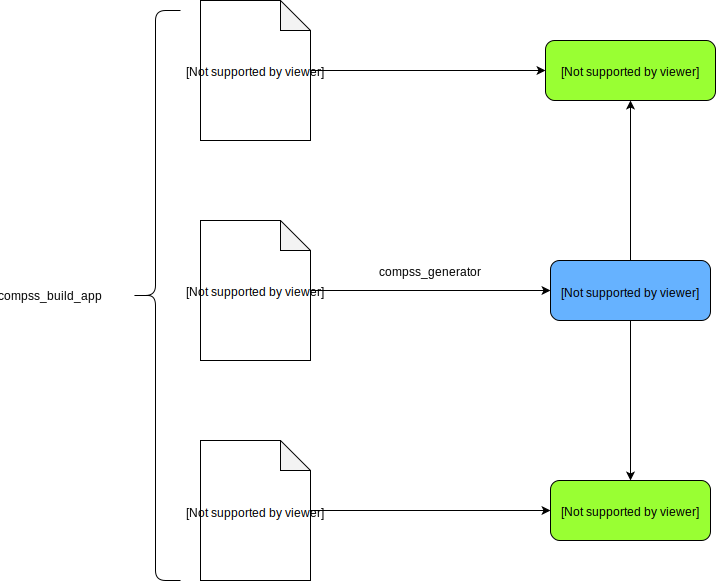
\includegraphics[width=\textwidth]{proceso_compilado.jpg}
    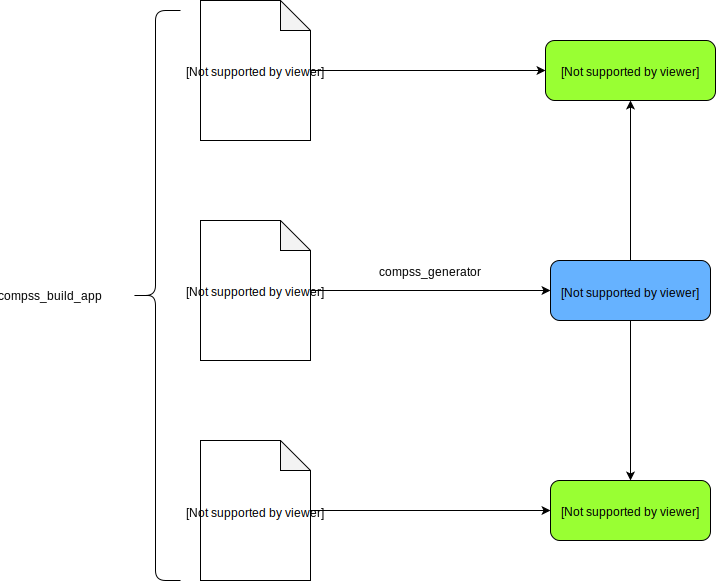
\includegraphics[scale=0.5]{proceso_compilado.jpg}
    \label{fig:proceso_compilado}
\end{figure}
\end{comment}

\subsection{Modelo de ejecución\label{modeloejecucion}}

El modelo de ejecución es sencillo, muy similar al modelo \textit{thread-pool}, al iniciar el \textit{runtime} se levanta el \textit{master} y un conjunto de \textit{workers}, a medida que se vayan generando tareas se estudiará qué \textit{workers} están libres y si cumplen los requisitos para ejecutar dicha tarea, y en ese caso la ejecutarán. 

\begin{figure}[H]
    \centering 
    \caption{Modelo de ejecución, basado en la aplicación 'ejemplo'.}
    %\includegraphics[width=\textwidth]{sta-masterworker.jpg}
    \includegraphics[scale=0.75]{sta-masterworker.jpg}
    \label{fig:masterworker_pool}
\end{figure}

La imagen muestra lo que sucede al ejecutar la aplicación de ejemplo de la sección \ref{compss_pm}, las líneas rojas curvas indican procesos (o bien \textit{threads}), lo importante sucede entre las flechas etiquetadas como compss\_on y compss\_off, la ejecución de la tarea. Se pide ejecutar la tarea funcionEjemplo al \textit{runtime} de \textit{COMPSs} y se decide en qué \textit{worker} se ejecutará. Hasta aquí podríamos pensar que es indéntico al \textit{thread-pool}. Nótese, que esto no es así, por el hecho de que no tenemos por qué hablar de una misma máquina, sino que pueden ser máquinas distintas, como se puede ver en el grupo de ordenadores de la imagen. 
\par\bigskip

En \textit{C/C++} existen dos tipos de \textit{worker}, uno \textbf{no persistente} y otro \textbf{persistente}. 

\begin{itemize}
 \item \textbf{No persistente:} Para cada tarea que se quiere ejecutar en uno de estos workers se debe crear el \textit{thread} y unas \textit{pipes} para hacer \textit{Inter-process communication} (IPC). %No sé si indagar en qué se pasa por las pipes, hmmm... qué se pasa por las pipes?
 \item \textbf{Persistente:} Este tipo de \textit{worker} se levanta una vez al inicio de la aplicación y espera recibir las tareas a ejecutar.
\end{itemize}


\section{OmpSs}

\textit{OmpSs} es desarrollado por el grupo \textit{PM - Programming Models}, perteneciente también al departamento de \textit{CS - Computer Science}.
\par\bigskip

\textit{OmpSs} es un modelo de programación que intenta explotar el paralelismo de las aplicaciones de una manera sencilla y aprovechando al máximo los recursos de la máquina\cite{duran2011ompss}. 
\par\bigskip
El nombre del modelo proviene de \textit{OpenMP} y \textit{StarSs} (modelo que desarrolló el \textit{BSC}), este integra funcionalidades presentes en ambos. Por parte de \textit{OpenMP} se quiere tomar la facilidad de paralelizar una aplicación secuencial insertando pragmas, y de \textit{StarSs} el modelo de ejecución basado en un \textit{thread-pool} y que permite la ejecución de código en más recursos que únicamente el procesador, es decir, que ofrece fácil gestión del resto de recursos de cómputo (\textit{GPUs}, \textit{FPGAs}, ...)\cite{sainz2014leveraging}\cite{filgueras2013heterogeneous}.

\subsection{Modelo de programación y ejecución}

El modelo de programación de \textit{OmpSs} se basa en la generación de tareas sencillamente insertando pragmas en código secuencial y a su vez facilitando la gestión de recursos heterogéneos. Veamos un pequeño ejemplo que muestre estas facultades.

\begin{minipage}{\linewidth}
\begin{lstlisting}[caption={Multiplicación de un bloque de una matriz utilizando GPUs.}, captionpos=b, label={lst:ompssmatmul.cc}, style=JStyle]
for (int i = 0; i < N; ++i) {
    for (int j = 0; j < N; ++j) {
        for (int k = 0; k < N; ++k) {
            #pragma omp target device(cuda) \
                               copy_deps    \
                               ndrange(2,N,N,32,32)
            #pragma omp task inout([N*N]C) in([N*N]A, [N*N]B)
            multiply_partitions_GPU(A[i*N+k], 
                                    B[k*N+j], 
                                    C[i*N+j], 
                                    n);
        }
    }
}
\end{lstlisting}
\end{minipage}

El código muestra una multiplicación de matrices por bloques. Con el primer pragma se indica que el dispositivo objetivo es una tarjeta gráfica que soporte \textit{CUDA}, y el segundo la declaración de una tarea y el tamaño de los bloques junto a las dependencias de esta.
\par\bigskip

El modelo de ejecución consiste en un \textit{thread-pool}, es decir, al generar tareas se escogerán \textit{threads} del \textit{pool} (entendámoslo como un conjunto de \textit{threads}) para ejecutarlas.
\par\bigskip

Cabe decir que para compilar una aplicación de \textit{OmpSs}, se utiliza el compilador \textit{source-to-source Mercurium} y el runtime \textit{Nanos++} para gestionar el paralelismo, es decir, la creación de tareas, sincronización entre estas, etc.

\section{Trabajo previo} 
\label{sec:compssompss}

Actualmente existe la posibilidad de desarrollar aplicaciones que utilicen \textit{OmpSs} dentro de \textit{COMPSs}. 
\par\bigskip
Para poder interactuar con el \textit{runtime} de \textit{OmpSs} \textit{Nanos++}, necesitamos gestionarlo nosotros manualmente o bien utilizar los \textit{pragmas} que nos propone el modelo de programación y compilar con \textit{Mercurium}. Entonces, asegurándonos de registrar los \textit{workers} en el \textit{runtime} y compilando su código fuente con \textit{Mercurium} aseguramos la interacción con el \textit{runtime} y por lo tanto la integración de ambos modelos.

Es posible desarrollar aplicaciones, como ya se ha comentado, pero con ciertas limitaciones. Dado que el worker \textit{no persistente}, se debe levantar para cada tarea, conseguimos aislar las tareas entre sí, cada tarea tendrá un \textit{runtime} de \textit{OmpSs} para el mismo, pero este mismo motivo añade mucho \textit{overhead} para la granularidad de las tareas de \textit{OmpSs}. El \textit{worker persistente} carece del \textit{overhead} de poner en marcha el \textit{runtime} de \textit{OmpSs}, pero también pierde la característica de aislar cada tarea del resto. Por una parte, no existe el \textit{overhead} que hay en el \textit{no persistente} pero el hecho de que no haya aislamiento provoca vale la pena ya que el \textit{worker} persiste durante la ejecución de la aplicación. Pese a que el \textit{persistente} mejora respecto al \textit{no persitente}, cuando se ejecutan varias tareas de \textit{COMPSs} que haga uso de \textit{OmpSs} en uno de estos \textit{workers} hay interferencias entre ellos.
\par\bigskip
El factor de aislamiento se vuelve todavía más crítico cuando en \textit{OmpSs} efectuar un \textit{taskwait} (\textit{pragma} que espera hasta que las tareas acaben) conlleva a que la espera se haga sobre todas las tareas de \textit{OmpSs} que estén en el \textit{runtime} por lo cual si no contamos con el aislamiento esperaremos a todas, hayan sido creadas o no por la misma tarea de \textit{COMPSs}. Para solucionarlo hay que efectuar accesos concurrentes sobre los datos que estemos tratando y hace que el \textit{taskwait} tenga como dependencia esos datos, así no esperaremos a absolutamente todas las tareas.
\par\bigskip
Estos problemas pretenden arreglarse integrando \textit{OmpSs-2}, que ofrece un \textit{runtime} nuevo llamado \textit{Nanos6} y nuevas características que vienen con este cambio como por ejemplo:

\begin{itemize}
\item \textbf{Liberación de las dependencias:} Las dependencias en esta versión se liberan de manera temprana, es decir, una vez una tarea acaba con un dato lo notifica al \textit{runtime} y este se encarga de notificar a las tareas que quedan libres de esta dependencia.
 \item \textbf{Relajación de las dependencias:} Ahora se pueden utilizar nuevos pragmas para determinar dependencias más suaves, no tan estrictas como en la versión anterior.
 \item \textbf{Ejecución de funciones de manera asíncrona:} La \textit{API} del nuevo \textit{runtime} \textit{Nanos6} permite ejecutar de manera asíncrona funciones en forma de tarea a partir de un puntero a una función, este método proporciona aislamiento del resto de tareas.
\end{itemize}

Hemos listado las que de alguna manera han sido clave para el proyecto, \textit{OmpSs-2} implementa muchas otras mejorías a parte de estas\cite{OmpSs2reference}. El proyecto estudia en las secciones \ref{sec:estudiopreviorend} y \ref{sec:estudiorend} si los problemas planteados han sido solucionados y el rendimiento que desempeña la nueva integración.

\section{Alcance del proyecto}

En esta sección se declaran las intenciones del proyecto (qué se pretende hacer), mediante una serie de requerimientos que harán que el proyecto pueda ser acabado con éxito, y unos objetivos que marcarán el desarrollo de este. También los posibles riesgos que surjan (y las soluciones de estos) y la metodología de trabajo que se llevará a cabo.

\subsection{Requerimientos}

 Los requerimientos necesarios para este proyecto son:

\begin{itemize}
 \item La nueva integración con \textit{OmpSs-2} no debe romper la actual compatibilidad con \textit{OmpSs}.
 \item El rendimiento de las aplicaciones desarrolladas con \textit{COMPSs+OmpSs-2} debe mejorar.
 \item Todas las modificaciones sobre \textit{COMPSs} deben ajustarse al grupo de \textit{Workflows and Distributed Computing}.
 \item Cualquier requerimiento impuesto (o aconsejado) por el \textit{BSC} formará parte de esta lista.
  
\end{itemize}

\subsection{Objetivos}

El objetivo principal de este proyecto es reformular la integración de \textit{COMPSs} con \textit{OmpSs} para solucionar los problemas actuales, ya sea integrándolo de nuevo pero esta vez con \textit{OmpSs-2} o bien idear otra manera de resolver las problemáticas. La siguiente lista muestra la posible descomposición de objetivos:

\begin{itemize}
  \item Aprender a utilizar la API (\textit{Application Programming Interface}) de \textit{Nanos6}.
  \item Eliminar o bien reducir las problemáticas planteadas en la sección   \ref{sec:compssompss}.
  \item Mejorar la gestión de recursos heterogéneos en las aplicaciones desarrolladas en \textit{COMPSs} integrando \textit{OmpSs-2}.
  \item En caso de conseguir el resto de objetivos plantear la integración en \textit{Java} y \textit{Python}.
\end{itemize}

\subsection{Riesgos}

Durante el desarrollo del proyecto pueden surgir problemas, para mejorar la reacción ante ellos listaremos los posibles riesgos y las respectivas soluciones.

\subsubsection{Problemas con el material de desarrollo}

Se podría romper el equipo en el cual se desarrolla el proyecto, pongamos que de una pantalla, un teclado y un ordenador se rompe el último. Se perdería todo el avance del proyecto, incluso documentación.
\par\medskip

\textbf{Solución:} Pese a que la pérdida del ordenador es importante, todo el código del proyecto será subido al \textit{GitLab} de \textit{WDS}, y la documentación al \textit{GitHub} personal del desarrollador, por lo cual se podría recuperar todo el  proyecto.

\subsubsection{Problemas con los clústers y supercomputadores}

Si por casualidad, caen los clústers y supercomputadores en los cuales se medirá el rendimiento del proyecto, se pararía la obtención de las métricas. 
\par\medskip

\textbf{Solución:} En este caso, como no resultaría lo mismo ejecutarlo en local en mi ordenador, debería optar por realizar otras tareas hasta que el equipo del \textit{BSC} solucione los inconvenientes.

\subsubsection{Aparición de errores en la implementación}

Cualquier proyecto esta lleno de errores en la implementación, hay que saber encontrarlos y solucionarlos lo más rápido posible, pero puede entorpecer el proyecto.
\par\medskip

\textbf{Solución:} Activaremos los \textit{flags} de \textit{debug} para poder evitar el mínimo error y en caso de su aparición utilizaremos \textit{gdb} (\textit{GNU Debugger}) para encontrarlo.

\subsubsection{Problemas con OmpSs/OmpSs-2}

Dado que se realizará una integración de otro proyecto del \textit{BSC} el desarrollador puede encontrarse con dificultades relacionadas con este a lo largo del proyecto.
\par\medskip

\textbf{Solución:} Después de haber intentado solucionarlo por sus propios medios se pondrá en contacto con el grupo de \textit{Programming Tools} con la descripción del error e intentos de solucionarlo.

\subsection{Metodología}

Para decidir la metodología a utilizar, hay que tener en cuenta que el proyecto consta únicamente de tres personas que se envolverán en él. El desarrollador, que hará todo el desarrollo tangible, el director y el co-director. 
\par\bigskip

La metodología que más se ciñe a las características del ``equipo'' es la iterativa. Consiste en planear las tareas a realizar y hacer una predicción de qué se conseguirá hacer en cortos periodos de tiempo llamados iteraciones. Además de estas predicciones, se consultará el estado del proyecto a menudo y se realizarán las tareas, una vez acabada una iteración empezará la siguiente, así hasta finalizar el proyecto.
\par\bigskip
Esta metodología nos permitirá reaccionar rápidamente a los imprevistos, además de hacer un bueno monitoreo del estado del proyecto, por lo cual se ha decidido emplearla.

\subsubsection{Herramientas}

Para efectuar el seguimiento del proyecto junto a mi director y codirector, se empleará un \textit{workspace} de \textit{Slack} para las comunicaciones directas (decidir dónde y cuándo hacer las reuniones por ejemplo), y \textit{Trello} para gestionar las tareas a desempeñar en cada iteración. Como ya se ha mencionado anteriormente, para el control de versiones del proyecto, código y documentación se utilizará respectivamente \textit{GitLab} y \textit{GitHub}.
\subsection{Herramientas}

Para efectuar el seguimiento del proyecto junto a mi director y co-director, se ha utilizado un \textit{workspace} de \textit{Slack} para las comunicaciones directas (para decidir dónde y cuándo hacer las reuniones por ejemplo), y \textit{Trello} para gestionar las tareas a desempeñar en cada iteración. Como ya se ha mencionado anteriormente, para el control de versiones del proyecto, código y documentación se ha utilizado respectivamente \textit{GitLab} y \textit{GitHub}.

%%%%%%%

\section{Planificación temporal}
\label{sec:planificacion}

Esta sección presenta cómo planificamos los cuatro meses de duración que tiene el proyecto, desde Febrero de 2019 hasta Junio de 2019 y cómo han sucedido realmente. Se especificarán las tareas a realizar junto a su durada aproximada y la duración que creemos que han tenido finalmente, también se han tenido en cuenta las posibles desviaciones en la realización de estas.

\subsection{Especificación de las tareas}

Detallamos a continuación las tareas a realizar.

\subsubsection{GEP - Gestión de proyectos}

La primera tarea del proyecto es la gestión de este, se han elaborado cuatro entregables que sintetizan la temática del proyecto, los objetivos, como se realizaría cuando se planificó y como se ha realizado, la metodología que se ha seguido, las actividades que se han realizado, y un estudio de sostenibilidad.

\begin{itemize}
 \item \textbf{Elaboración del primer entregable:} En este primer apartado se  un contexto, el estado del arte del proyecto, los objetivos, requerimientos, riesgos y una metodología para desarrollar el proyecto en sí. La duración aproximada es de unas 24 horas.
 \item \textbf{Elaboración del segundo entregable:} En este apartado se definen las actividades y duración de estas. La duración aproximada es de 6 horas.
 \item \textbf{Elaboración del tercer entregable:} En este apartado se ha realizado la auto-evaluación sobre la sostenibilidad además de un análisis sobre la gestión económica y la sostenibilidad del proyecto. La duración aproximada es de 18 horas.
 \item \textbf{Elaboración del cuarto entregable:} En este último apartado se ha preparado una presentación oral y se ha confeccionado el documento final, que serán los tres anteriores revisados y corregidos con la orientación del \textit{feedback} del profesor de \textit{}, director y co-director. La duración aproximada es de 12 horas.
\end{itemize}

Con estos cuatro apartados se finaliza el primer bloque de tareas. En princpio, la duración estipulada del GEP es de 75 horas, la duración final ha sido de 60 horas por lo que tuvimos tiempo para revisar y repasar estos apartados.

\par\bigskip

Para realizar esta actividad, se ha utilizado un ordenador, \textit{GitHub} para subir la documentación, \textit{Kile} para redactar el documento en \textit{LaTeX},\textit{Trello} para organizar las actividades en forma de tarjetas, \textit{Gantter} para elaborar el diagrama de \textit{Gantt} y \textit{Google Drive}.

\subsubsection{Uso de la API de Nanos6}

Para poder llevar acabo exitosamente la integración, se necesita entender qué hace y saber utilizar la \textit{API} de \textit{Nanos6}. Requiere mirar documentación e interactuar con los desarrolladores de \textit{Nanos6}. 
\par\bigskip

Hemos aprendido a utilizar la llamada \textit{nanos6\_spawn\_function}, que nos permite ejecutar una función como tarea. Para poder utilizarla, necesitamos levantar el \textit{runtime} de manera manual en un programa compilado con \textit{gcc} (\textit{GNU C Compiler}) o bien \textit{g++} cuando se utilice \textit{C++}, y efectuar la llamada a una función externa compilada con \textit{mcc} (\textit{Mercurium}), ya que estará anotada con pragmas de \textit{OmpSs-2}.
\par\bigskip

La duración de esta tarea ha sido de 60 horas. Los recursos necesarios son un ordenador con un compilador nativo de \textit{C}, otro de \textit{C++}, y \textit{Mercurium} y \textit{Nanos6} instalados. 

\subsubsection{Integrar OmpSs-2 en el binding de C/C++}

La tarea principal que da sentido al proyecto es esta, comprende el estudio y la integración de \textit{OmpSs-2} en el \textit{binding} de \textit{C/C++}. Requiere del estudio de la estructura interna de \textit{COMPSs} por una banda y del \textit{binding} por otra, hemos tenido que decidir dónde se puede inicializar el \textit{runtime} de \textit{Nanos6} y cuándo se debe apagar. También se necesita hacer la llamada a la \textit{API} en el \textit{worker}, cosa que ha habido que estudiar dónde situar dentro del código.
\par\bigskip

El primer paso ha consistido en analizar dónde tiene más sentido que hagamos la gestión del \textit{runtime} de \textit{Nanos6}, y cómo hacerla. Para se ha repasado el código de \textit{COMPSs} y se ha determinado qué hace cada componente de este. 
%\par\bigksip

En segundo lugar se ha implementado toda la gestión. Claro que también ha habido que efectuar la llamada a la \textit{API} y verificar el funcionamiento de la integración, ha sido lo que más tiempo nos ha llevado sin duda alguna.
%\par\bigskip

Esta tarea ha sido la que más tiempo nos ha llevado, pero nos ha conocimiento pleno de cómo funciona el modo librería y el \textit{binding} de\textit{C/C++}. La duración ha estado alrededor de 96 horas. Los recursos necesarios han sido un ordenador con \textit{COMPSs} instalado, un compilador nativo de \textit{C}, otro de \textit{C++}, y \textit{Mercurium} y \textit{Nanos6} instalados.

\subsubsection{Estudiar la integración de OmpSs-2 en Java y binding de Python}

\begin{comment}
En caso de que la primera integración haya funcionado, se estudiará la posibilidad de hacer lo mismo con \textit{Java} y el \textit{binding} de \textit{Python}. Consistirá exactamente de los mismos pasos, y puede ayudar a mejorar la implementación anterior. La duración estimada de esta tarea dependerá de si se decide realizar o no esta actividad. Mínimo se emplearán 15 horas en el estudio preliminar, y en caso de realizar la integración, 78 horas más, es decir, 15 horas o bien 93 horas. Pese a que la tarea es muy similar a la anterior, el tiempo previsto es algo menor por el hecho de que ya se ha podido realizar una integración y la implementación debería ser parecida. Los recursos necesarios son un ordenador con \textit{COMPSs} instalado, un compilador nativo de \textit{C}, otro de \textit{C++}, y \textit{Mercurium} y \textit{Nanos6} instalados.
\end{comment}

Finalmente esta tarea se descartó, fue preferible invertir tiempo en el resto de funcionalidades y evaluar la integración de la mejor manera posible. Aún así, se invirtió tiempo en sopesar posibilidades para realizar tanto la integración de \textit{Java} como la de \textit{Python}, por lo que la duración ha sido alrededor de 15 horas.

\subsubsection{Desarrollo de una aplicación que use COMPSs+OmpSs-2}

En esta tarea se han desarrollado dos aplicaciones, \textit{K-Means} y \textit{Cholesky} utilizando \textit{COMPSs+OmpSs-2}, se han utilizado para evaluar el rendimiento en otra tarea. Hemos empleado aproximadamente 84 horas en desarrollar ambas aplicaciones y testear que funcionasen. Los recursos necesarios son un ordenador con \textit{COMPSs} instalado, un compilador nativo de \textit{C}, otro de \textit{C++}, y \textit{Mercurium} y \textit{Nanos6} instalados

\subsubsection{Estudio del rendimiento}

Utilizando las aplicaciones desarrolladas en la tarea anterior hemos estudiado el rendimiento de la integración. Se ha hecho uso de opciones de \textit{COMPSs} para medir cuánto tarda cada tarea enviada a un nodo. 
\par\bigskip

Estudiar el rendimiento ha incluido intentar optimizar al máximo todas las pérdidas de rendimiento en la medida de lo posible, por lo cual el tiempo aproximado para llevarla a cabo, ha sido de 84 horas. Los recursos necesarios son un ordenador con \textit{COMPSs} instalado, un compilador nativo de \textit{C}, otro de \textit{C++}, y \textit{Mercurium} y \textit{Nanos6} instalados.

\subsubsection{Limitaciones de COMPSs+OmpSs-2}

Dado que este proyecto parte de la premisa de resolver unos problemas concretos con el rendimiento, se efectúa un estudio muy concreto hacia estos problemas para ver si están resueltos o no. Que este estudio vaya mal o no, no afecta realmente al proyecto, ya que se intentará ver si \textit{OmpSs-2} mejora respecto a \textit{OmpSs} de todas formas.

\subsubsection{Redactar la memoria}

Por último se ha redactado la memoria del proyecto además de preparar todo el material audiovisual para la defensa de este. La duración de esta actividad ha sido de unas 72 horas. Los recursos que utilizados son \textit{Kile} para redactar el documento en \textit{LaTeX}, \textit{GitHub} para guardar la documentación y \textit{LibreOffice} para el apoyo audiovisual que se utilizará durante la defensa.

\subsection{Dependencias}

La siguiente tabla define la relación de dependencia entre las tareas que conciernen a la gestión del proyecto.

\begin{table}[H]
\centering
 \begin{tabular}{|| l | l ||}
    \hline  
    Tarea dependiente & Tarea predecesora \\
    \hline\hline
    Contexto & - \\
    \hline
    Estado del arte & Contexto \\
    \hline
    Objetivos, requerimentos, riesgos & Estado del arte \\
    \hline
    Metodología & Objetivos, requerimentos, riesgos \\
    \hline
    Definir actividades & Metodología \\
    \hline
    Estimar tiempos & Definir actividades \\
    \hline
    Autoevaluación sobre la sostenibilidad & Estimar tiempos \\
    \hline
    Análisis del proyecto & Autoevaluación sobre la sostenibilidad \\
    \hline
    Confeccionar documento final & Análisis del proyecto \\
    \hline
    Preparar presentación & Confeccionar documento final \\
    \hline
 \end{tabular}
 \caption{Relación de dependencia para las tareas de la gestión del proyecto.}
 \label{table:1}
\end{table}

La tabla anterior muestra la relación de dependencia, se respetará esta relación ya que las tareas a elaborar se agrupan y tienen fecha de entrega por separado. 

\begin{table}[H]
 \centering
 \begin{tabular}{|| l | l ||}
    \hline  
    Tarea dependiente & Tarea predecesora \\
    \hline\hline
    Uso de la API Nanos6 & GEP \\
    \hline
    Integrar OmpSs-2 en C/C++ & Uso de la API \\
    \hline
    Integrar OmpSs-2 en Java & Integrar OmpSs-2 en C/C++ \\
    \hline
    Integrar OmpSs-2 en Python & Integrar OmpSs-2 en Java \\
    \hline
    Estudio previo del rendimiento & Integrar OmpSs-2 en Python \\
    \hline
    Desarrollo aplicación COMPSs+OmpSs-2 & Estudio previo del rendimiento \\
    \hline
    Estudio del rendimiento & Desarrollo aplicación COMPSs+OmpSs-2 \\
    \hline
    Redactar la memoria & Estudio del rendimiento \\
    \hline
 \end{tabular}
    \caption{Relación de dependencia para las tareas de implementación del proyecto.}
    \label{table:2}
\end{table}

Salvo por algún motivo que implique bloquear una tarea, no se deberán adelantar tareas dependientes a las predecesoras, entre estos posibles motivos se contemplan errores en la implementación que nos bloqueen y se puedan ir haciendo otras cosas y cambios generales en las tareas a realizar.

\subsection{Estimación temporal de las tareas y recursos necesarios}

En el momento en el que se han enumerado y explicado las tareas se ha comentado la duración temporal y los recursos necesarios para cada actividad. En las siguientes dos secciones se recopilan estos datos en forma de tabla.

\subsection{Estimación temporal de las tareas}

\begin{table}[H]
 \centering
 \begin{tabular}{|| l | l ||}
  \hline
  Tarea & Estimación temporal (horas) \\
  \hline\hline
   Gestión del proyecto & 60 \\%& GitHub, Kile, Trello, Gantter, Google Drive \\
   \hline
   Uso de la API Nanos6 & 60 \\%& Compilador de C y C++, Mercurium, Nanos6 \\
   \hline
   Integrar OmpSs-2 en C/C++ & 96 \\%& COMPSs, Compilador de C y C++, Mercurium, Nanos6 \\
   \hline
   Integrar OmpSs-2 en Java y Python & 93 \\%& COMPSs, Compilador de C y C++, Mercuirum, Nanos6 \\
   \hline
   Desarrollo aplicación COMPSs+OmpSs-2 & 84 \\%& COMPSs, Compilador de C y C++, Mercurium, Nanos6 \\
   \hline
   Estudio del rendimiento & 84 \\%& COMPSs, Compilador de C y C++, Mercurium, Nanos6 \\
   \hline
   Redactar la memoria & 72 \\%& GitHub, Kile, LibreOffice \\
  \hline
  Total & 549 \\
  \hline
 \end{tabular}
 \caption{Estimación temporal de las tareas.}
\end{table}

\subsection{Duración real de las tareas}

Todas las tareas han durado lo esperado a excepción de la tarea que consiste en realizar la integración de \textit{OmpSs-2} en \textit{Java} y \textit{Python}, nos hemos limitado a hacer el estudio preliminar, por lo que ha durado 15 horas.

\begin{table}[H]
 \centering
 \begin{tabular}{|| l | l ||}
  \hline
  Tarea & Estimación temporal (horas) 			\\
  \hline\hline
   Gestión del proyecto & 60 					\\
   \hline
   Uso de la API Nanos6 & 60 					\\
   \hline
   Integrar OmpSs-2 en C/C++ & 96 				\\
   \hline
   Integrar OmpSs-2 en Java y Python & 15 		\\
   \hline
   Desarrollo aplicación COMPSs+OmpSs-2 & 84 	\\
   \hline
   Estudio del rendimiento & 84 				\\
   \hline
   Redactar la memoria & 72 					\\
  \hline
  Total & 471 									\\
  \hline
 \end{tabular}
 \caption{Estimación temporal de las tareas.}
\end{table}

\subsection{Recursos necesarios para las tareas}

\begin{table}[H]
 \centering
 \begin{tabular}{| l | l |}
 \hline
 Tarea & Recursos necesarios \\
 \hline\hline  
 Gestión del proyecto & GitHub, Kile, Trello, Gantter, Google Drive \\
 \hline
 Uso de la API Nanos6 & Compilador de C y C++, Mercurium, Nanos6 \\
 \hline
 Integrar OmpSs-2 en C/C++ & COMPSs, Compilador de C y C++, Mercurium, Nanos6 \\
 \hline
 Integrar OmpSs-2 en Java y Python & COMPSs, Compilador de C y C++, Mercurium, Nanos6 \\
 \hline
 Estudio del rendimiento & COMPSs, Compilador de C y C++, Mercurium, Nanos6 \\
 \hline
 Redactar la memoria & GitHub, Kile, LibreOffice \\
 \hline
 \end{tabular}
 \caption{Recursos necesarios para las tareas.}
\end{table}

En la tabla anterior, se muestran los recursos estrictamente necesarios para realizar cada tarea, sin embargo, se ofrece ahora una lista de los recursos \textit{hardware} y \textit{software} que se han utilizado para la realización del proyecto en general. Además hay que tener en cuenta todos los recursos humanos necesarios.

\subsubsection{Recursos hardware}

\begin{itemize}

 \item \textbf{Ordenador portátil:} Proporcionado por el \textit{BSC}, Dell Latitude 7480 Intel® Core™ i7-6650U Processor (Dual Core, 4M Cache, 2.2GHz,15W, vPro), 512GB SSD (\textit{Solid State Drive}), Intel® HD Graphics 540 y 16 GB de memoria \textit{RAM}.
 
 \item \textbf{Pantalla:} Es habitual la configuración de portátil con una pantalla para simular una torre, la pantalla externa es también Dell, el modelo Professional P2217H.
 
 \item \textbf{Periféricos:} Todos los periféricos, ratón y teclado en este caso.
 
 \item \textbf{Clústers:} Con tal de medir el rendimiento ejecutando la aplicación que se ha desarrollado haciendo uso de la integración, necesitaremos un clúster con una arquitectura heterogénea. En la lista de candidatos se encontraban \textit{MinoTauro} y \textit{CTE-Power}, pero al final se descartó \textit{MinoTauro} por problemas de compatibilidad y se utilizó \textit{MareNostrum4}
 
 \item \textbf{Puesto de trabajo:} El equipo de \textit{WDC} se encuentra en el edificio \textit{K2M}, allí es donde el desarrollador tiene su puesto de trabajo y ha desarrollado la mayoría del proyecto.
 
\end{itemize}

\subsubsection{Recursos software}

\begin{itemize}
    \item \textbf{Ubuntu 18.04:} Con tal de desarrollar se necesita un sistema operativo, el portátil tiene instalado \textit{Ubuntu 18.04}.

    \item \textbf{GitHub y GitLab:} Para efectuar un control de versiones sencillo y eficaz, se ha utilizado el \textit{GitHub} personal del desarrollador para gestionar la documentación y el \textit{GitLab} del grupo \textit{WDC} para gestionar el código.

    \item \textbf{Editores: } Para editar código en \textit{Java} se ha utilizado \textit{IntelliJ IDEA}, para \textit{Python} \textit{PyCharm}, ambos de \textit{JetBrains}, y para C y C++ se ha usado \textit{Vim}.

    \item \textbf{Terminal: } La gran parte del tiempo ha estado entre terminales haciendo implementaciones y probando su funcionamiento, para hacer uso de un terminal utilizamos el emulador de terminales \textit{Terminator}.

    \item \textbf{Planificación y organización: } Para hacer el diagrama de \textit{Gantt} se ha utilizado \textit{Gantter} como extensión para \textit{Google Drive}. Además para organizarse y emplear la metodología iterativa se utilizará \textit{Trello}.

    \item \textbf{Compiladores y gestores de proyectos: } Para compilar código en C y C++ se usa \textit{gcc} y \textit{g++} respectivamente, para todo código que use \textit{OmpSs-2} se ha utilizado \textit{Mercurium}. El proyecto de \textit{COMPSs} está gestionado con \textit{Maven}, de esta manera se pueden generar todos los ficheros de \textit{Java} de manera sencilla. 
    
    \item \textbf{Software del proyecto: } Para poder desarrollar el proyecto, se precisa de una instalación de \textit{COMPSs}, \textit{Nanos6} y \textit{Mercurium}. Además, para medir el rendimiento se utiliza \textit{Extrae} y \textit{Paraver}. Con fines de \textit{debugging} se ha utilizado \textit{gdb}.

    \item \textbf{Editores de texto: } Para escribir el \textit{LaTeX} se utiliza \textit{Kile}.
\end{itemize}

\subsubsection{Recursos humanos}

\begin{itemize}
 \item \textbf{Director y co-director: } Han efectuado el seguimiento del proyecto de manera rutinaria y han ayudado a que el desarrollador sea capaz de llevarlo a cabo. 
 \item \textbf{Soporte: } Al utilizar \textit{software} de diversos proyectos, todas las personas que han ayudado al desarrollador a solucionar problemas han sido recursos necesarios del proyecto.
 \item \textbf{Desarrollador: } Persona encargada de llevar a cabo en última instancia el proyecto.
\end{itemize}

\subsection{Valoración de alternativas y plan de acción}

En un proyecto de este tipo, es probable que haya desviaciones respecto el plan original. Esto es normal, tan sólo hay que saber cómo actuar ante estas desviaciones. Cualquier error en una implementación puede acarrear tiempo de más para solucionarlo, e incluso algo que se implementó hace mucho puede influir en las del futuro, por ello nuestra planificación intenta ser flexible, aún así, debemos planear como actuar en estos casos.

\begin{itemize}
 \item Si una tarea dura menos de lo esperado, sencillamente hay que coger la siguiente de la planificación y empezar a hacerla. Que una tarea dure menos que otra nos puede aportar un margen de acción muy útil.
 \item Si una tarea dura más tiempo de lo esperado, habrá que planteárselo de dos maneras, o bien se acorta otra tarea con tal de ajustarnos a la planificación o bien se intentan reducir lo mínimo posible los objetivos del proyecto para poderlo acabar en el tiempo establecido.
\end{itemize}

La tarea que más tiempo puede llevar dada la aparición de imprevistos es la de integrar \textit{OmpSs-2} en el \textit{binding} de C. Dado que la documentación aún está en una fase un tanto primeriza y no siempre tenemos por qué contar con el apoyo de soporte, por lo cuál habrá que invertir tiempo extra en ese caso. 
\par\medskip
El resto de tareas van un poco de la mano de esta anterior, no debería haber ninguna complicación extra. Como mucho en el estudio del rendimiento podemos encontrar resultados que no nos gusten o no acaben de agradar del todo, pero es parte del proyecto, se intentará mejorar dentro del tiempo estipulado. 
\par\medskip
Por tanto, siempre que falte tiempo para realizar una tarea se intentará equilibrar entre el resto, ya que el riesgo de sufrir un imprevisto es bastante bajo.
\par\bigskip
Para ser más previsores, en las reuniones de seguimiento se intentarán prever estos posibles problemas durante la realización del proyecto. 

De hecho, en un punto del proyecto descubrimos que \textit{MinoTauro} no era compatible con \textit{OmpSs-2} si queríamos hacer uso de las \textit{GPUs}, por esto tuvimos que rectificar y decidir utilizar \textit{MareNostrum4} y sacar provecho tan sólo de las \textit{CPUs}. También, el hecho de no haber realizado la integración en \textit{Java} y \textit{Python} supone de alguna manera una desviación, pero ya estaba prevista.



















\section{Gestión económica y de sostenibilidad del proyecto}
\label{sec:sostenibilidad}
\subsection{Autoevaluación sobre la sostenibilidad}

Todos los alumnos que hayan realizado un trabajo de final de grado este cuatrimestre, saben qué supone el impacto de un proyecto sobre la sostenibilidad. Es difícil para mí, analizar de manera crítica y de alguna manera metódica estos impactos que se describen en la encuesta. 
\par\medskip
En cuanto a conocer los impactos, tener sentido común e intentar siempre reducir los impactos que de alguna manera sean insostenibles, sí que hay un conocimiento pleno y ganas de mantenerlo, pero desconozco los métodos más avanzados y profesionales para abordar la reducción de impactos negativos y aumentar la sostenibilidad de un proyecto.
\par\medskip
Los aspectos ambientales son de alguna manera los que resultan más intuitivos, de manera que no resulta difícil desenvolverse en primer momento, pero no conozco en profundidad el tema.
\par\medskip
En cuánto a aspectos sociales, de igual manera que los ambientales, soy capaz de reconocer cuando un proyecto impacta de manera negativa en la sociedad (que puede suceder aunque aparentemente parezca beneficioso en primer momento). Pero cuando se trata de poner sobre la mesa un estudio preciso sobre estos aspectos, no soy capaz, desconozco la teoria.
\par\medskip
Sobre aspectos económicos es donde más fallo, pese a que tengo cierta formación gracias a asignaturas impartidas en la \textit{FIB}, me resulta complicado entender y comprender como a mí me gustaría estos aspectos. Aún así tengo la voluntad y las ganas de ser capaz de analizarlo de manera correcta.
\par\medskip
Básicamente, se quiere poder analizar de igual manera los tres aspectos, ambiental, social y económico, existe una voluntad fehaciente que por desgracia puede resultar insuficente cuando se ahonda en el análisis.

\subsection{Gestión económica y sostenibilidad}

%Cuando se desarrolla un proyecto siempre hay un cierto impacto ambiental, económico, social. Cómo el proyecto impacta sobre estas tres componentes indica cuánto de sostenbile es el proyecto. Aunque \textit{a priori} desconocemos las técnicas para medir el impacto, se conseguirá hacer una aproximación del impacto del proyecto. 

%\subsection{Análisis de la sostenibilidad}

A lo largo de esta sección, se detallará la gestión económica del proyecto. Se estudiarán los costes tanto directos e indirectos y las posibles desviaciones en términos económicos. Además se estudiará también el componente que queda olvidado en la mayoría de proyectos informáticos, la sostenibilidad de este.

\subsubsection{Costes directos e indirectos}

Los costes directos de este proyecto, vienen a partir de los recursos definidos para el proyecto y las actividades que se llevan a cabo en este. Es importante tener en cuenta que por mucho que los recursos tenga un coste directo en el proyecto y estén asociados a este, los recursos tienen una vida útil por lo cuál habrá un grado de amortización del coste por recurso. Estos costes se recapitulan a continuación en forma de tabla.

\begin{table}[ht!]
\centering
 \begin{tabular}{| l | l | l | l | l |}
    \hline
    Unidades & Unidad & Precio/Unidad(\euro) & Vida útil (años) & Amortización (\euro/h) \\
    \hline
    \cline{1-1}
    \rowcolor{gray!50}
    Recursos hardware \\
    \hline
    Dell Latitude 7480          & 1 & 1500  & 4 & 0.21\\
    \hline 
    Dell Professional P2217H    & 1 & 250   & 4 & 0.03\\
    \hline
    Periféricos                 & 1 & 50    & 4 & 0.07\\
    \hline
    \rowcolor{gray!50}
    Total                       & - & 0     & - & 0.31\\
    \hline
    \cline{1-1}
    \rowcolor{gray!50}
    Recursos software \\
    \hline
    Ubuntu 18.04                & 1 & 0     & - & 0\\
    \hline
    GitHub                      & 1 & 0     & - & 0\\
    \hline
    GitLab                      & 1 & 0     & - & 0\\
    \hline
    Terminator                  & 1 & 0     & - & 0\\
    \hline
    Gantter                     & 1 & 0     & - & 0\\
    \hline
    Trello                      & 1 & 0     & - & 0\\
    \hline
    Google Drive                & 1 & 0     & - & 0\\
    \hline
    Kile                        & 1 & 0     & - & 0\\
    \hline
    LibreOffice                 & 1 & 0     & - & 0\\
    \hline
    Maven                       & 1 & 0     & - & 0\\
    \hline
    GNU Compiler Collection     & 1 & 0     & - & 0\\
    \hline
    GDB                         & 1 & 0     & - & 0\\
    \hline
    Extrae                      & 1 & 0     & - & 0\\
    \hline
    Paraver                     & 1 & 0     & - & 0\\
    \hline
    OmpSs-2                     & 1 & 0     & - & 0\\
    \hline
    COMPSs                      & 1 & 0     & - & 0\\
    \hline
    \rowcolor{gray!50}
    Total                       & - & 0     & - & 0\\
    \hline
 \end{tabular}
\caption{Costes directos divididos en recursos hardware y software.}
\end{table}

Los recursos \textit{GitHub}, \textit{IntelliJ IDEA} y \textit{PyCharm}, no añaden ningún coste al proyecto ya que se utilizan versiones y subscripciones para estudiantes. Por otra parte \textit{Gantter} proporciona una versión de prueba de 30 días, por lo cuál tampoco añade ningún coste.
\par\bigskip

En la anterior tabla se han omitido los dos clústers, ya que querríamos costearlos a \euro$/$h y no por unidad. Se puede considerar que \textit{MareNostrum4} y \textit{CTE-Power} no suponen ningún coste al proyecto, ni de adquisición de este ni eléctrico, ya que son proporcionados por el \textit{BSC}, aún así para proporcionar una visión más realista se ha seleccionado una máquina de \textit{Amazon Web Services} \textit{AWS} con características similares a cada clúster, con tal de seleccionar un precio \euro$/$h adecuado. Para \textit{MareNostrum4} se ha considerado que la instancia de modelo \textit{r5.12xlarge} a un coste de 2.7 \euro/h, y para \textit{CTE-Power} la instancia \textit{Amazon EC2 P3} modelo \textit{p3.8xlarge} a un coste de 10.85 \euro/h.
\par\bigskip

En cuanto a costes directos solo nos falta comentar los que provienen de los recursos humanos del proyecto.

\begin{comment}
begin{table}[ht!]
 \centering
 \begin{tabular}{c|c|c|c|} 
  \cline{2-4}
                & Horas (h) & Precio/Hora(\euro) & Total(\euro) \\
  \cline{2-4}\hline
  Desarrollador & 489 & 10 & 4890 \\
  \hline
  Director & 55 & 30 & 1650\\
  \hline 
  Codirector & 50 & 30 & 1500\\
  \hline
  Soporte & 20 & 20 & 400\\
  \hline
  \rowcolor{gray!50}
  Total & - & - & 8440\\
  \hline
 \end{tabular}
\caption{Costes directos provenientes de recursos humanos.}
\end{table}
\end{comment}

\begin{table}[ht!]
\begin{tabular}{l|l|l|l|}
\cline{2-4}
                                                    & Horas (h) & Precio/Hora(\euro) & Total(\euro) \\ \hline
\multicolumn{1}{|l|}{Desarrollador}                 & 489       & 10               & 4890     \\ \hline
\multicolumn{1}{|l|}{Director}                      & 55        & 30               & 1650     \\ \hline
\multicolumn{1}{|l|}{Codirector}                    & 50        & 30               & 1500     \\ \hline
\multicolumn{1}{|l|}{Soporte}                       & 20        & 20               & 400      \\ \hline
\rowcolor{gray!50}
\multicolumn{1}{|l|}{Total} &    -       &  -              &  8440        \\ \hline
\end{tabular}
\caption{Costes directos provenientes de recursos humanos.}
\end{table}

Es difícil cuantificar las horas que entran en soporte, dado que este puede ser efectuado por varias personas con distintos sueldos, se ha optado por pensar que se dedicará un total de 20 horas y que el prefio esta en la media entre un desarrollador y un director.

\par\bigskip

Los costes indirectos del proyecto engloban el alquiler de la oficina (edificio K2M) el gasto energético de esta , su debido mantenimiento la contratación de servicios como internet, u otros servicios que se ofrezcan al conjunto de trabajadores en general. Del enlace \cite{k2msuperficie} se extrae que la superfície de la primera planta del edifico K2M es de $445,6 m^{2}$ y de \cite{k2mpreu} que el coste para una empresa es de 17.8 \euro$/m^{2}$ al mes. El gasto en consumo eléctrico de la planta se da por hecho que entra en el precio estipulado por el alquiler.
% preu https://govern.upc.edu/ca/consell-de-govern/consell-de-govern/sessio-3-2017-de-consell-de-govern/aprovacio-de-la-modificacio-de-les-tarifes-dels-espais-parc-upc/9-11-modificacio-de-les-tarifes-desl-espais-parc-upc.pdf/@@display-file/visiblefile/9.11%20Modificaci%C3%B3%20de%20les%20tarifes%20desl%20espais%20Parc%20UPC.pdf
% superficie https://wwwbupc.webs.upc.edu/bupc/hemeroteca/2008/b107/05-06-2008.pdf

\begin{table}[ht!]
\begin{tabular}{l|l|l|l|l|}
\cline{2-5}
                                                    & Meses   & $m^{2}$ & Precio mensual(\euro$/m^{2})$ & Total(\euro) \\ \hline
\multicolumn{1}{|l|}{Alquiler oficinas }            & 4  & 445,6   & 17,8 & 31.726,72     \\ \hline
\rowcolor{gray!50}
\multicolumn{1}{|l|}{Total} & - &   -       &  -              &   31.726,72       \\ \hline
\end{tabular}
\caption{Costes indirectos derivados del alquiler de las oficinas.}
\end{table}

\subsection{Imprevistos y contingencias}

En la planificación temporal se tuvo en cuenta que todos los proyectos sufren de desviaciones e imprevistos. Las desviaciones pueden ser anticipadas efectuando las reuniones de seguimiento, pero los imprevistos son inevitables. Evidentemente, ante la aparición de cualquiera de estos dos, habría un aumento de los costes directos e indirectos (el tiempo dedicado por los recursos humanos aumenta, por lo tanto el coste, etc).
\par\medskip
En la siguiente sección, se detallarán los costes a nivel de recurso y uso temporal de estos por cada actividad a desarrollar en el proyecto. Con tal de no proponer un presupuesto que pueda quedar negativo por culpa de imprevistos, se dedicará un porcentaje extra de las tareas a poder sobrevenir el posible coste.
En el mejor de los casos no tendremos imprevistos o bien será una cantidad tan pequeña que el porcentaje extra reservado por tarea nos permitirá costearnos los imprevistos. Por otra banda, si tenemos un imprevisto con cada tarea es muy posible que no seamos capaces de cubrir los costes (en función del porcentaje que se reserve, claro).

\subsection{Presupuesto}


\begin{longtable}{l|l|l|l|l|l|}
\cline{2-6}

                                                                                                                                    & Uds.                            	& Precio(\euro o \euro/h)         	& Vida útil(años)        			 		& Amortización(\euro/h)       		& Precio(\euro)                       \\ \hline
\endfirsthead
%
\endhead
%
\rowcolor[HTML]{9B9B9B} 
\multicolumn{1}{|l|}{\cellcolor[HTML]{9B9B9B}Costes directos}                                                                       &                                 &                         &                         &                         & {\color[HTML]{343434} 17.034,58} \\ \hline
\rowcolor[HTML]{C0C0C0} 
\multicolumn{1}{|l|}{\cellcolor[HTML]{C0C0C0}{\color[HTML]{343434} Gestión del proyecto}}                                           & {\color[HTML]{343434} 60 horas} & {\color[HTML]{343434} } & {\color[HTML]{343434} } & {\color[HTML]{343434} } & {\color[HTML]{343434} 620,45}   \\ \hline
\multicolumn{1}{|l|}{Dell Latitude 7480}                                                                                            & 1                               & 1500                    & 4                       & 0,2841                  & 17,05                           \\ \hline
\multicolumn{1}{|l|}{Dell Professional P2217H}                                                                                      & 1                               & 250                     & 4                       & 0,0473                  & 2,84                            \\ \hline
\multicolumn{1}{|l|}{Periféricos}                                                                                                   & 1                               & 50                      & 4                       & 0,0095                  & 0,57                            \\ \hline
\multicolumn{1}{|l|}{Ubuntu 18.04}                                                                                                  & 1                               & 0                       & -                       & -                       & 0                               \\ \hline
\multicolumn{1}{|l|}{GitHub}                                                                                                        & 1                               & 0                       & -                       & -                       & 0                               \\ \hline
\multicolumn{1}{|l|}{Gantter}                                                                                                       & 1                               & 0                       & -                       & -                       & 0                               \\ \hline
\multicolumn{1}{|l|}{Trello}                                                                                                        & 1                               & 0                       & -                       & -                       & 0                               \\ \hline
\multicolumn{1}{|l|}{Google Drive}                                                                                                  & 1                               & 0                       & -                       & -                       & 0                               \\ \hline
\multicolumn{1}{|l|}{Kile}                                                                                                          & 1                               & 0                       & -                       & -                       & 0                               \\ \hline
\multicolumn{1}{|l|}{LibreOffice}                                                                                                   & 1                               & 0                       & -                       & -                       & 0                               \\ \hline
\multicolumn{1}{|l|}{Desarrollador}                                                                                                 & 1                               & 10                      & -                       & -                       & 600                             \\ \hline
\rowcolor[HTML]{C0C0C0} 
\multicolumn{1}{|l|}{\cellcolor[HTML]{C0C0C0}Uso de la API Nanos6}                                                                  & 60 horas                        &                         &                         &                         & 620,45                          \\ \hline
\multicolumn{1}{|l|}{Dell Latitude 7480}                                                                                            & 1                               & 1,500                    & 4                       & 0,2841                  & 17,05                           \\ \hline
\multicolumn{1}{|l|}{Dell Professional P2217H}                                                                                      & 1                               & 250                     & 4                       & 0,0473                  & 2,84                            \\ \hline
\multicolumn{1}{|l|}{Periféricos}                                                                                                   & 1                               & 50                      & 4                       & 0,0095                  & 0,57                            \\ \hline
\multicolumn{1}{|l|}{OmpSs-2}                                                                                                       & 1                               & 0                       & -                       &                         & 0                               \\ \hline
\multicolumn{1}{|l|}{COMPSs}                                                                                                        & 1                               & 0                       & -                       & -                       & 0                               \\ \hline
\multicolumn{1}{|l|}{GNU Compiler Collection}                                                                                       & 1                               & 0                       & -                       & -                       & 0                               \\ \hline
\multicolumn{1}{|l|}{Desarrollador}                                                                                                 & 1                               & 10                      & -                       & -                       & 600                             \\ \hline
\rowcolor[HTML]{C0C0C0} 
\multicolumn{1}{|l|}{\cellcolor[HTML]{C0C0C0}Integrar OmpSs-2 en C/C++}                                                             & 96 horas                        &                         &                         &                         & 992,72                          \\ \hline
\multicolumn{1}{|l|}{Dell Latitude 7480}                                                                                            & 1                               & 1,500                    & 4                       & 0,2841                  & 27,27                           \\ \hline
\multicolumn{1}{|l|}{Dell Professional P2217H}                                                                                      & 1                               & 250                     & 4                       & 0,0473                  & 4,54                            \\ \hline
\multicolumn{1}{|l|}{Periféricos}                                                                                                   & 1                               & 50                      & 4                       & 0,0095                  & 0,912                           \\ \hline
\multicolumn{1}{|l|}{OmpSs-2}                                                                                                       & 1                               & 0                       & -                       & -                       & 0                               \\ \hline
\multicolumn{1}{|l|}{COMPSs}                                                                                                        & 1                               & 0                       & -                       & -                       & 0                               \\ \hline
\multicolumn{1}{|l|}{GNU Compiler Collection}                                                                                       & 1                               & 0                       & -                       & -                       & 0                               \\ \hline
\multicolumn{1}{|l|}{Desarrollador}                                                                                                 & 1                               & 10                      & -                       & -                       & 960                             \\ \hline
\rowcolor[HTML]{C0C0C0} 
\multicolumn{1}{|l|}{\cellcolor[HTML]{C0C0C0}\begin{tabular}[c]{@{}l@{}}Integrar OmpSs-2 en Python\\ y Java\end{tabular}}           & 93 horas                        &                         &                         &                         & 961,7                           \\ \hline
\multicolumn{1}{|l|}{Dell Latitude 7480}                                                                                            & 1                               & 1,500                    & 4                       & 0,2841                  & 26,42                           \\ \hline
\multicolumn{1}{|l|}{Dell Professional P2217H}                                                                                      & 1                               & 250                     & 4                       & 0,0473                  & 4,40                            \\ \hline
\multicolumn{1}{|l|}{Periféricos}                                                                                                   & 1                               & 50                      & 4                       & 0,0095                  & 0,88                            \\ \hline
\multicolumn{1}{|l|}{OmpSs-2}                                                                                                       & 1                               & 0                       & -                       & -                       & 0                               \\ \hline
\multicolumn{1}{|l|}{COMPSs}                                                                                                        & 1                               & 0                       & -                       & -                       & 0                               \\ \hline
\multicolumn{1}{|l|}{GNU Compiler Collection}                                                                                       & 1                               & 0                       & -                       & -                       & 0                               \\ \hline
\multicolumn{1}{|l|}{Desarrollador}                                                                                                 & 1                               & 10                      & -                       & -                       & 930                             \\ \hline
\rowcolor[HTML]{C0C0C0} 
\multicolumn{1}{|l|}{\cellcolor[HTML]{C0C0C0}\begin{tabular}[c]{@{}l@{}}Desarrollo de una aplicación\\ COMPSs+OmpSs-2\end{tabular}} & 84 horas                        &                         &                         &                         & 868,63                          \\ \hline
\multicolumn{1}{|l|}{Dell Latitude 7480}                                                                                            & 1                               & 1500                    & 4                       & 0,2841                  & 23,86                           \\ \hline
\multicolumn{1}{|l|}{Dell Professional P2217H}                                                                                      & 1                               & 250                     & 4                       & 0,0473                  & 3,97                            \\ \hline
\multicolumn{1}{|l|}{Periféricos}                                                                                                   & 1                               & 50                      & 4                       & 0,0095                  & 0,80                            \\ \hline
\multicolumn{1}{|l|}{OmpSs-2}                                                                                                       & 1                               & 0                       & -                       & -                       & 0                               \\ \hline
\multicolumn{1}{|l|}{COMPSs}                                                                                                        & 1                               & 0                       & -                       & -                       & 0                               \\ \hline
\multicolumn{1}{|l|}{GNU Compiler Collection}                                                                                       & 1                               & 0                       & -                       & -                       & 0                               \\ \hline
\multicolumn{1}{|l|}{Desarrollador}                                                                                                 & 1                               & 10                      & -                       & -                       & 840                             \\ \hline
\rowcolor[HTML]{C0C0C0} 
\multicolumn{1}{|l|}{\cellcolor[HTML]{C0C0C0}Estudio del rendimiento}                                                               & 84 horas                        &                         &                         &                         & 12.250,63                        \\ \hline
\multicolumn{1}{|l|}{Dell Latitude 7480}                                                                                            & 1                               & 1,500                    & 4                       & 0,2841                  & 23,86                           \\ \hline
\multicolumn{1}{|l|}{Dell Professional P2217H}                                                                                      & 1                               & 250                     & 4                       & 0,0473                  & 3,97                            \\ \hline
\multicolumn{1}{|l|}{Periféricos}                                                                                                   & 1                               & 50                      & 4                       & 0,0095                  & 0,80                            \\ \hline
\multicolumn{1}{|l|}{MareNostrum4}                                                                                                     & 10                              & 2,7                    & -                       & -                       & 2268,0                          \\ \hline
\multicolumn{1}{|l|}{CTE-Power}                                                                                                     & 10                              & 10,85                   & -                       & -                       & 9,114                            \\ \hline
\multicolumn{1}{|l|}{OmpSs-2}                                                                                                       & 1                               & 0                       & -                       & -                       & 0                               \\ \hline
\multicolumn{1}{|l|}{COMPSs}                                                                                                        & 1                               & 0                       & -                       & -                       & 0                               \\ \hline
\multicolumn{1}{|l|}{GNU Compiler Collection}                                                                                       & 1                               & 0                       & -                       & -                       & 0                               \\ \hline
\multicolumn{1}{|l|}{Extrae}                                                                                                        & 1                               & 0                       & -                       & -                       & 0                               \\ \hline
\multicolumn{1}{|l|}{Paraver}                                                                                                       & 1                               & 0                       & -                       & -                       & 0                               \\ \hline
\multicolumn{1}{|l|}{Desarrollador}                                                                                                 & 1                               & 10                      & -                       & -                       & 840                             \\ \hline
\rowcolor[HTML]{C0C0C0} 
\multicolumn{1}{|l|}{\cellcolor[HTML]{C0C0C0}Redactar la memoria}                                                                   & 72 horas                        &                         &                         &                         & 720                             \\ \hline
\multicolumn{1}{|l|}{GitHub}                                                                                                        & 1                               & 0                       & -                       & -                       & 0                               \\ \hline
\multicolumn{1}{|l|}{Kile}                                                                                                          & 1                               & 0                       & -                       & -                       & 0                               \\ \hline
\multicolumn{1}{|l|}{LibreOffice}                                                                                                   & 1                               & 0                       & -                       & -                       & 0                               \\ \hline
\multicolumn{1}{|l|}{Desarrollador}                                                                                                 & 1                               & 10                      & -                       & -                       & 720                             \\ \hline
\rowcolor[HTML]{9B9B9B} 
\multicolumn{1}{|l|}{\cellcolor[HTML]{9B9B9B}Costes indirectos}                                                                     &                                 &                         &                         &                         & 31.726,72                        \\ \hline
\multicolumn{1}{|l|}{Alquiler oficinas K2M}                                                                                         & -                               & -                       & -                       & -                       & 31.726,72                        \\ \hline
\multicolumn{1}{|l|}{Servicios}                                                                                                     & -                               & -                       & -                       & -                       & -                               \\ \hline
\rowcolor[HTML]{9B9B9B} 
\multicolumn{1}{|l|}{\cellcolor[HTML]{9B9B9B}Total acumulado}                                                                       &                                 &                         &                         &                         & 48.761,3                         \\ \hline
\rowcolor[HTML]{9B9B9B} 
\multicolumn{1}{|l|}{\cellcolor[HTML]{9B9B9B}Contingencia}                                                                          & 10\%                            &                         &                         &                         & 53.637,43                        \\ \hline
\rowcolor[HTML]{9B9B9B} 
\multicolumn{1}{|l|}{\cellcolor[HTML]{9B9B9B}Total sin IVA}                                                                         &                                 &                         &                         &                         & 53.637,43                        \\ \hline
\rowcolor[HTML]{9B9B9B} 
\multicolumn{1}{|l|}{\cellcolor[HTML]{9B9B9B}Total con IVA}                                                                         & 21\%                            &                         &                         &                         & 64.901,29                        \\ \hline
\end{longtable}

En la anterior tabla de detalla el presupuesto final del proyecto, se define la contingencia y se aplica el impuesto \textit{IVA}. En esta última tabla no siempre se ha hecho referencia a todos los recursos, esto ha sido así siempre que el recurso tuviera un papel secundario (por ejemplo editores o terminales, que son cosas a elección del desarrollador...) y el coste fuera nulo.

\begin{comment}
\subsection{Dimensión económica}

\begin{itemize}
 \item \textbf{Reflexión sobre el coste estimado para la realización del proyecto.}\newline
 
    El presupuesto ha sido elaborado de manera cautelosa y más bien conservadora, intentando llegar a cubrir todos los gastos y siendo previsores añadiendo el margen de contingencia. En la mayoría de actividades los recursos principales con coste no nulo son el equipo informático y el propio desarrollador, por lo cual ante cualquier imprevisto serán los recursos que añadirán más costes.

 \item \textbf{Como se resuelve actualmente el problema que quieres abordar? En que mejorará económicamente tu solución respecto a las existentes?}\newline
 
 El problema actualmente se aborda de diversas maneras, el problema es que estas son costosas en términos de tiempo, se pretende aportar una nueva manera de resolverlo que ahorre en términos de tiempo, que se traduce en dinero.
\end{itemize}

\subsection{Dimensión ambiental}

\begin{itemize}
 \item \textbf{Has estimado el impacto ambiental que tendrá la realización del proyecto?}\newline
 
 Es difícil estimar el impacto ambiental, en este tipo de proyectos no estamos creando una cadena de montaje ni aplicando un nuevo método para facilitar algún proceso industrial. El impacto de nuestro proyecto recae en el consumo energético de las máquinas en las que se medirá en rendimiento, y una vez puesto en producción todo el consumo energético que generen el resto de proyectos que utilicen como recurso el nuestro. Por otra parte es interesante tener en cuenta que nuestro proyecto pretende poder aprovechar al máximo los recursos de cómputo de una plataforma, de tal manera se consumirá más pero de una manera más eficiente, por tanto, mejor.
 
 \item \textbf{Te has planteado minimizar el impacto, por ejemplo, reutilizando recursos?}\newline
 
 Todos los recursos utilizados tanto software como hardware pueden ser reutilizados hasta que la vida útil de estos recursos finalice.
 
 \item \textbf{Como se resuelve actualmente el problema que quieres abordar? En que mejorará ambientalmente tu solución respecto a las existentes?}\newline
 
Como se ha dicho anteriormente, hay diversas maneras de abordar el problema, el caso es que no se cree que mejore ambientalmente respecto al resto, será interesante de igual manera intentar efectuar una medición del consumo energético  bien la eficiencia energética.
\end{itemize}

\subsection{Dimensión social}

\begin{itemize}
 \item \textbf{Qué crees que te aportará a nivel personal la realización del proyecto?}\newline
 
 El proyecto me dará una nueva visión del mundo de la investigación, ya que en ciertos momentos trabajaré codo con codo con los mejores en el campo. Además me aportará conocimientos diversos de los modelos de programación paralelos y distribuidos, y su funcionamiento interno.
 \item \textbf{Cómo se resuelve actualmente el problema que quieres abordar? En que mejorará socialmente tu solución respecto a las existentes?}\newline
 
 Este proyecto puede ser utilizado al final para desarrollar aplicaciones que envuelvan campos de carácter social (tanto médico, como literalmente social...). Aún así, no supone ninguna mejoría respecto a lo que aportan el resto de soluciones a nivel social.
 
 \item \textbf{Existe una necesidad real del proyecto?}\newline
 
 Abordando la pregunta desde una perspectiva social no existe la necesidad para el ciudadano del proyecto. La comunidad científica sí que puede aprovecharse de la facilidad que aportará el proyecto al desarrollo de aplicaciones en entornos heterogéneos distribuidos.
 
\end{itemize}
\end{comment}

\section{Informe de sostenibilidad}

\subsection{Dimensión ambiental}

\begin{itemize}
	\item \textbf{¿Has cuantificado el impacto ambiental de la realización del proyecto? ¿Qué medidas has
		tomado para reducir el impacto? ¿Has cuantificado esta reducción?} \\
	
	Por desgracia no ha habido tiempo para cuantificar el impacto ambiental del proyecto. Se podría haber estimado el consumo de energía de \textit{CTE-Power} y \textit{MareNostrum4} al ejecutar los experimentos, en caso de haberlo estimado, las únicas medidas posibles para reducir el impacto hubieran sido minimizar el uso de estas máquinas, usarlas solo cuando estuviera completamente seguro que el experimento iba a funcionar, de esta manera el consumo se reduciría drásticamente a utilizar todos los recursos desde 1 a 10 nodos en ambas máquinas. 
	
	\item \textbf{¿Si hicieras de nuevo el proyecto, ¿Podrías realizarlo con menos recursos?} \\
	
	Desde luego podría haber invertido menos tiempo conociendo de antemano qué me depara en cada fase del proyecto, pero los recursos utilizados son estrictamente los necesarios, no falta ni sobra ninguno.
	
	\item \textbf{¿Qué recursos estimas que se usarán durante la vida útil del proyecto? ¿Cuál será el
		impacto ambiental de estos recursos?} \\
	
	Es difícil conocerlo, durante la vida útil del proyecto puede ser utilizado en clústers y supercomputadores de manera que los recursos no son pocos, pero el proyecto no hace uso de recursos por si solo, siempre será en el contexto de otro proyecto o investigación científica. Quizá el único recurso estricto es mantener las versiones del proyecto en la nube con controles de versión como \textit{GitHub} o \textit{GitLab}, donde el impacto ambiental viene derivado del consumo de sus servidores.
	
	\item \textbf{¿El proyecto permitirá reducir el uso de otros recursos? ¿Globalmente, el uso del proyecto
		mejorará o empeorará la huella ecológica?} \\
	
	El proyecto pretende facilitar la programación en entornos distribuidos heterogéneos, por lo que el tiempo que se utilizarán estos entornos se verá reducido, por lo cual estaremos ayudando a reducir los recursos de otros proyectos. Definitivamente, el uso del proyecto mejorará la huella ecológica.
	
	\item \textbf{¿Podrían producirse escenarios que hiciesen aumentar la huella ecológica del proyecto?} \\
	
	La huella ecológica del proyecto durante el desarrollo podría verse afectada en el caso que hubiera un desvío notorio en las fases de experimentación donde hay que utilizar máquinas que suponen un consumo energético elevado. \textit{A posteriori} no puede ser que se aumente la huella ecológica intrínseca del proyecto, la posible huella viene dada por el uso que los usuarios hagan del proyecto.
	
	
\end{itemize}

\subsection{Dimensión económica}

\begin{itemize}
	
	\item \textbf{\textbf{¿Has cuantificado el coste (recursos humanos y materiales) de la realización del proyecto? ¿Qué decisiones has tomado para reducir el coste? ¿ Has cuantificado este ahorro?}} \\
	
	Se ha cuantificado el coste de recursos humanos y materiales durante la realización del proyecto, para reducir el coste de los recursos humanos se ha intentado hacer las reuniones con el director y co-director las veces justas, minimizar el uso de recursos humanos solo cuando sea estrictamente necesario, para los recursos materiales se ha intentado utilizar una porción de las máquinas asequible y se ha intentado minimizar el uso de estas. Estas medidas se han tomado desde el primer momento por lo que el presupuesto ya se ajusta a ellas, no ha habido ningún ahorro al respecto.
	
	\item \textbf{¿Se ha ajustado el coste previsto al coste final? ¿Has justificado las diferencias (lecciones aprendidas)?} \\
	
	El coste se ha visto afectado en el hecho que tuvimos que descartar el uso del \textit{MinoTauro} por que las tarjetas gráficas que utilizan son incompatibles con los \textit{drivers} más nuevos de \textit{NVIDIA} por lo que \textit{OmpSs-2} no las soporta. Para reemplazar la máquina decidimos utilizar \textit{MareNostrum4}, lo que nos llevo a aumentar el coste final. Pero el coste previsto del proyecto aparte de la desviación que comentada no ha sufrido ningún desajuste, se ajusta completamente.
	
	\item \textbf{¿Qué coste estimas que tendrá el proyecto durante su vida útil? ¿ Se podría reducir este
		coste para hacerlo más viable?} \\
	
	El proyecto no tiene ningún coste una vez desarrollado, si hubiera uno sería coste de infraestructura para mantenerlo en la nube de \textit{GitHub} o \textit{GitLab} pero es un servicio gratuito para instituciones de carácter público. El coste no se puede reducir más.
	
	\item \textbf{¿Se ha tenido en cuenta el coste de los ajustes/actualizaciones/reparaciones durante la
		vida útil del proyecto?} \\
	
	No, dado que es una pieza de \textit{software} que integra dos modelos de programación no debería necesitar de actualizaciones durante su vida útil que no vengan hechas por los propios equipos de desarrollo de \textit{COMPSs} o \textit{OmpSs-2}, aún así, si hiciera falta se añadió el porcentaje de contingencia para poder encarar situaciones similares.
	
	\item \textbf{¿Podrían producirse escenarios que perjudicasen la viabilidad del proyecto?} \\
	
	El proyecto no pretende lucrarse por lo que realmente la viabilidad no podría verse afectada. La integración \textit{COMPSs+OmpSs-2} pretende ser utilizada en el marco de investigaciones científicas.
	
\end{itemize}

\subsection{Dimensión social}

\begin{itemize}
	\item \textbf{¿La realización de este proyecto ha implicado reflexiones significativas a nivel personal, profesional o ético de las personas que han intervenido?} \\
	
	Por suerte el proyecto no ha llevado a ninguna persona implicada a tener que reflexionar de esta manera. Las reflexiones realizadas han sido sólo en el marco definido única y exclusivamente por el proyecto.
	
	\item \textbf{¿Quién se beneficiará del uso del proyecto?} \\
	
	Todo usuario que lo utilice, principalmente destinado a personal de investigación que quiera programar en entornos distribuidos heterogéneos de una manera más sencilla y efectiva.
	
	\item \textbf{¿Hay algún colectivo que puede verse perjudicado por el proyecto? ¿ En qué medida?} \\
	
	Desde luego que no, el proyecto no puede afectar de ninguna manera a ningún colectivo, podría afectar a nivel competitivo pero no tiene como objetivo ser vendido en el mercado y cuenta con licencias que permiten su uso, modificación y distribución de manera gratuita.
	
	\item \textbf{¿En qué medida soluciona el proyecto el problema planteado inicialmente?} \\
	
	El proyecto soluciona el problema tal y como estaba planeado desde que se inició la gestión del proyecto.
	
	\item \textbf{¿Podrían producirse escenarios que hiciesen que el proyecto fuese perjudicial para algún
		segmento particular de la población?} \\
	
	El proyecto por si mismo no supone ninguna amenaza para ningún segmento de la población, solo el uso que le den los usuarios podría ser perjudicial. Pero no creo que seamos responsables del uso que hagan los usuarios cuando brindamos una herramienta que únicamente pretende hacer más fácil la programación de entornos distribuidos heterogéneos.
	
	\item \textbf{¿Podría crear el proyecto algún tipo de dependencia que dejase a los usuarios en posición
		de debilidad?} \\
	
	De ninguna manera. El proyecto no incluye características que creen dependencia entre este y el usuario, en caso de que alguien desarrollase este tipo de dependencia sería un caso muy particular a tratar.
	
\end{itemize}





\usepackage{xr}
\externaldocument{GEP/deliverable1.tex}

\section{Integración de OmpSs-2 en C/C++ COMPSs}

Con tal de realizar una buena integración necesitamos conocer bien cómo funcionan y/o cómo están hechos los componentes a integrar. Con tal de adquirir los conocimientos necesarios, vamos a indagar en la estructura interna del \textit{binding} de \textit{C/C++} de \textit{COMPSs} y a entender cómo se desarrolla y compila una aplicación. También deberemos ver cómo funciona la \textit{API} del \textit{runtime} de \textit{OmpSs-2} \textit{Nanos6} y el proceso habitual de desarrollo y compilado de una aplicación que utiliza el modo librería.

\subsection{Estructura de los bindings}

El \textit{runtime} de \textit{COMPSs} fue desarrollado en \textit{Java}, por lo que si queremos soportar cualquier lenguaje (salvo el propio \textit{Java}), necesitamos de alguna manera establecer comunicación con ese lenguaje. Es decir, necesitaremos un mecanismo que nos permita ejecutar código de este lenguaje a soportar, por supuesto, en ambas direcciones. 
\par\bigskip
Actualmente, \textit{COMPSs} cuenta con los \textit{bindings} de \textit{C/C++} y \textit{Python} (usualmente conocido como \textit{PyCOMPSs}), que utilizan estos mecanismos descritos anteriormente. Para efectuar la ejecución entre \textit{Java} y \textit{C/C++} se utiliza la \textit{Java Native Interface}, dado que desde \textit{Python} se puede utilizar la \textit{Python-C API} para , con un componente intermedio entre \textit{Python} y \textit{Java} escrito en \textit{C/C++} (utilizando la \textit{JNI}) permitiríamos efectuar llamadas desde \textit{C/C++} y \textit{Python} al \textit{runtime} y al revés. 
\par\bigskip
La siguiente imagen muestra la estructura general de los \textit{bindings} actuales. Las cajas representan componentes de la arquitectura, el color de cada caja ha sido escogido para representar un lenguaje, por lo que dos cajas del mismo color que estén conectadas directamente con un flecha no requieren de mecanismos adicionales.

\begin{figure}[H]
    \centering 
    \caption{Estructura de los bindings de COMPSs.}
    %\includegraphics[width=\textwidth]{sta-masterworker.jpg}
    \includegraphics[scale=0.6]{estructuraBindings.png}
    \label{fig:estructura_bindings}
\end{figure}

\subsection{Modelo de ejecución en el binding C/C++}

\textit{C} y \textit{C++} son lenguajes de programación compilados, esto quiere decir que necesitamos un segundo programa llamado compilador que procese nuestro programa y genere un fichero que nuestro ordenador pueda ejecutar, a este proceso se le llama compilar y al fichero generado, binario. De esta manera, para poder obtener el modelo de ejecución introducido en la sección \ref{modeloejecucion}, necesitaremos compilar dos binarios, uno para el \textit{master} y otro para los \textit{workers}.
\par\bigskip

\begin{comment}
La aplicación que desarrolla el usuario, \textit{a priori} no envía las tareas a ejecutar ni las dependencias entre estas, no gestiona el \textit{runtime}, pero es desarrollada siguiendo unas directrices que nos permitirán generar código que sí gestione todo lo que es necesario con tal de que la aplicación se distribuya correctamente. 
\end{comment}

La aplicación que desarrolle el usuario, tiene que ser transparente al \textit{runtime}, para conseguirlo tan sólo se necesita una interfaz indicando las tareas a detectar al ejecutar la aplicación. Entonces, una vez compilemos la aplicación de COMPSs en C/C++, se generará automáticamente (a partir de ahora \textit{autogenerar}) código para las tareas, que gestionarán la comunicación con el \textit{runtime}.
\smallskip
La siguiente imagen describe de manera visual cómo se compila una aplicación. 

\begin{figure}[H]
    \centering 
    \caption{Proceso de compilación de una aplicación COMPSs C/C++.}
    %\includegraphics[width=\textwidth]{sta-masterworker.jpg}
    \includegraphics[scale=0.6]{workflowCompilado.png}
    \label{fig:workflowcompilado}
\end{figure}

\par\bigskip
Para facilitar el compilado de la aplicación se utiliza el script \textit{compss\_build\_app}, y para hacer la generación de código a partir de la interfaz, el binario \textit{compss\_generator}.
\par\bigksip

La aplicación una vez desarrollada por el usuario, compilada sin \textit{COMPSs} por el medio también funcionaría, pero sencillamente las tareas serían ejecutadas \textit{in situ} en el \textit{master}.  Lo que pretendemos hacer al introducir \textit{COMPSs} es que el \textit{master}, en vez de ejecutar la tarea, comunique al \textit{runtime} que se debe ejecutar una tarea, y este se encargue de ejecutarla en un \textit{worker}, todo evidentemente, de manera transparente al usuario.
\par\bigskip












\section{Evaluación}
\label{sec:estudiorend}

En esta sección describiremos las aplicaciones descritas para evaluar la integración \textit{COMPSs+OmpSs-2}, los entornos donde haremos la evaluación y los resultados de esta.  

\subsection{Aplicaciones}
\subsubsection{K-Means}

\textit{K-Means} es un algoritmo utilizado para hacer \textit{clustering} sobre un grupo de datos, es decir, agrupar los datos en \textit{clusters}. Cada dato pertenece al \textit{cluster} cuyo centro está en la distancia mínima, si no fuera así pertenecería a otro \textit{cluster}. Se inicializan \textit{clusters} con centros escogidos de manera aleatoria y se comparan las distancias a todos los \textit{clusters} y se determina a cual pertenece cada dato (siempre al centro más cercano), una vez hecho esto se vuelve a calcular el centro de cada \textit{cluster}, todo este proceso conforma una iteración de \textit{K-Means}, habitualmente se itera hasta que converge, esto es que la distancia entre los centros asignados en dos interaciones consecutivas de cada \textit{cluster} es cercana a 0.
\par\bigskip
Tal y como hemos desarrollado la aplicación tiene 4 tareas, que son \textit{init\_Fragment}, \textit{compute\_newCluster} (tiene una implementación en CPU y otra en GPU), \textit{merge\_newCluster}, \textit{update\_Clusters}. El siguiente grafo de dependencias muestra una ejecución de \textit{K-Means} con 5 fragmentos de 25 dimensiones con 200000 puntos cada uno, el número de \textit{clusters} a formar es 25 y se efectúa una única iteración. Para no sobrecargar este apartado se incluye en el apéndice \ref{sec:codigokmeans} la interfaz y el programa principal de la aplicación.

\begin{figure}[H]
	\centering 
	\caption{Grafo de dependencias entre tareas de K-Means.}
	\includegraphics[scale=0.2]{grafo_kmeans.pdf}
	\label{fig:grafokmeans}
\end{figure}

\subsubsection{Cholesky}

\textit{Cholesky} es un método de descomposición aplicable cuando la matriz es simétrica definida positiva, entonces esta puede ser descompuesta como el producto de una matriz triangular inferior y su traspuesta. El método \textit{Cholesky} se utiliza para resolver sistemas de ecuaciones lineales, es similar a la descomposición \textit{LU} y es el doble de eficiente, la única restricción es que no siempre es aplicable.
\par\bigskip
La aplicación ha sido desarrollada utilizando una librería para operaciones de algebra lineal programada en \textit{C} con \textit{OmpSs} y \textit{OmpSs-2}, esta librería es \textit{LASs}\footnote{https://pm.bsc.es/mathlibs/lass} (\textit{Linear Algebra routines on OmpSs}). Las funciones que implementa \textit{LASs} serán utilizadas como tareas a nivel de \textit{COMPSs} y después una vez ejecutadas harán uso de \textit{OmpSs-2}, por lo que realmente desarrollar una aplicación utilizando una librería externa es muy sencillo.
\par\bigskip
Tiene 5 tareas, son \textit{generate\_block}, \textit{ddss\_dpotrf}, \textit{ddss\_dtrsm}, \textit{ddss\_dgemm}, \textit{ddss\_dsyrk}, la primera se utiliza para generar los bloques de manera distribuida (así el \textit{master} no tiene reservar memoria para toda la matriz, que podría ser muy grande), y las otras 4 son operaciones de algebra lineal que utilizadas de la forma correcta aplicarán el método de descomposición de \textit{Cholesky}. En el apéndice \ref{sec:codigocholesky} se encuentra la interfaz y el prorgama principal del programa.

\todo{grafo cholesky}

\subsection{Entornos para el estudio}

Para la realización del estudio del rendimiento se han utilizado dos máquinas que el \textit{Barcelona Supercomputing Center} pone a nuestra disposición, que son \textit{CTE-Power} y \textit{MareNostrum4}.

\subsubsection{CTE-Power}
\label{sec:power}

\textit{CTE-Power} es un \textit{cluster} basado en la tecnología de procesadores \textit{IBM} \textit{Power9}. Tiene 2 nodos de \textit{login}, son los nodos desde donde operan los usuarios y 52 nodos de cómputo. 
\par\smallskip
Cada nodo tiene los siguientes componentes:
\par\smallskip
\begin{itemize}
	\item 2 x \textit{IBM Power9 8335-GTH} @ 2.4GHz (3.0GHz en modo turbo), cada procesador con 20 cores cada uno con 4 \textit{threads}.
	\item 512GB de memoria organizada en 16 \textit{dimms} de 32GB @ 2666MHz.
	\item 4 x \textit{NVIDIA} V100 con 16GB \textit{HBM2}.
	\item 2 x SSD que proporcionan 1.9TB de almacenaje local.
	\item 2 x \textit{NVM Express} 3.2TB.
	\item Interfaz de red \textit{Mellanox}.
	\item Sistema de ficheros GPFS a través de fibra a 10GBit.
\end{itemize}

Nosotros utilizaremos tan sólo 10 nodos, por lo que tendremos a nuestra disposición en la mayor ejecución 1600 CPUs y 40 GPUs \textit{NVIDIA V100}. 

\subsubsection{MareNostrum4}
\label{sec:mare}

\textit{MareNostrum4} es un supercomputador basado en la tecnología de procesadores \textit{Intel Xeon Platinum} de la generación \textit{Skylake}. Tiene 5 nodos de \textit{login} y 3.456 nodos de cómputo.
\par\smallskip
Cada nodo tiene los siguientes componentes:
\par\smallskip
\begin{itemize}
	\item 2 x \textit{Intel Xeon Platinum 8160 @ 2.10GHz} con 24 cores.
	\item 96 GB de memoria organizada en 12 \textit{dimms} de 8GB @ 2667MHz.
	\item Un SSD que proporciona 200 GB de almacenaje local.
	\item 100 Gbit/s \textit{Intel Omni-Path HFI Silicon 100 Series PCI-E adapter}.
	\item 10 Gbit \textit{Ethernet}.
\end{itemize}

Igual que con \textit{CTE-Power} tan sólo utilizaremos 10  nodos, por lo tanto tendremos en la mayor ejecución 480 CPUs.

\subsection{K-Means}

La evaluación con \textit{K-Means} ha consistido en hacer un test de \textit{strong scaling}, que consiste en ejecutar la aplicación con un tamaño de problema fijo y aumentar el número de recursos de cómputo, y otro de \textit{weak scaling} donde aumentaremos de manera proporcional el tamaño del problema y los recursos de cómputo. En el apartado \ref{sec:power} describimos la máquina que utilizamos en estos test, haremos uso de todas las \textit{CPUs} y \textit{GPUs} de cada nodo.

\subsubsection{Strong scaling}

La imagen \ref{fig:sc-time} muestra una gráfica que tiene en el eje vertical el tiempo y en el horizontal el número de nodos. El tamaño del problema que se ha utilizado es de 400 fragmentos de 50 dimensiones y 200000 puntos cada uno, el número de \textit{clusters} a formar es 50 y se efectúan 5 iteraciones. Se han tomado 10 muestras de cada ejecución, la línea azul muestra la media de las muestras para el mismo número de nodos, la de color naranja muestra el tiempo ideal que debería tardar según el número de nodos. En cada punto de la línea azul se muestra la diferencia entre el máximo valor y el mínimo que se han tomado en las muestras.

\begin{figure}[H]
	\centering 
	\caption{Tiempo de ejecución al aumentar el número de recursos.}
	\includegraphics[scale=0.8]{estudio/KMeans/sc/kmeans-sc-time.png}
	\label{fig:sc-time}
\end{figure}

Es bueno que la línea azul sea lo más parecida a la línea naranja, eso nos indicaría que la aplicación escala perfectamente, ya que cada vez que aumentamos los recursos el tiempo de ejecución se reduciría proporcionalmente. La imagen \ref{fig:sc-speedup} muestra la misma información que \ref{fig:sc-time} dispuesta en forma de ganancia, se puede ver que se comporta bien hasta que en los 6 nodos empieza a dejar de acercarse al ideal.

\begin{figure}[H]
	\centering 
	\caption{Ganancia al aumentar el número de recursos.}
	\includegraphics[scale=0.8]{estudio/KMeans/sc/kmeans-sc-speedup.png}
	\label{fig:sc-speedup}
\end{figure}

\subsubsection{Weak scaling}

En un test de \textit{weak scaling}, esperamos que los tiempos de ejecución sean siempre los mismos, ya que el tamaño del problema es siempre proporcional a los recursos de cómputo. Esto sería perfecto pero hay que efectuar comunicación entre nodos y gestionar todo el sistema, por lo que no podemos mantener este escenario ideal. La imagen \ref{fig:wc-effic} muestra cómo al aumentar el número de nodos la eficiencia baja del ideal (que el tiempo de ejecución sea siempre el mismo), pero se mantiene alrededor del mismo valor a partir de los 6 nodos.

\begin{figure}[H]
	\centering 
	\caption{Eficiencia al mantener proporcional el tamaño del problema y el número de recursos.}
	\includegraphics[scale=0.8]{estudio/KMeans/wc/kmeans-wc-efficiency.png}
	\label{fig:wc-effic}
\end{figure}

\subsection{Cholesky}











\appendixpage
\appendix
\begin{landscape}

\section{Planificación y diagrama de Gantt correspondiente}

\begin{figure}[H]
    \centering 
    \caption{Tareas definidas para el diagrama de Gantt.}
    \includegraphics[scale=2.5]{ganttProyecto.png}
    \label{fig:gantt_tareas}
\end{figure}

\begin{figure}[H]
    \centering 
    \caption{Diagrama de Gantt del proyecto.}
    \includegraphics[scale=2]{diagramaGantt.png}
    \label{fig:diagrama_gantt}
\end{figure}
\end{landscape}

\externaldocument{technical_work/ompss-2-integration.tex}

\section{Pthreads y mecanismos de sincronización}
\label{appendix:pthread}

En este apéndice se introduce superficialmente qué es un \textit{Pthread} y se hace hincapié en el mecanismo utilizado para la sincronización con las tareas registradas en \textit{Nanos6} con el modo librería introducido en la sección \ref{spawnfunction}
\bigskip

Históricamente los \textit{threads} se han implementado por cada fabricante o empresa, de una manera específica, complicando la portabilidad entre plataformas. Los \textit{Pthreads} nos proveen un estándar con la intención de que sea utilizado por la mayoría de máquinas. En todos los sistemas operativos del tipo \textit{UNIX} se implementan los \textit{threads} con el estándar \textit{IEEE POSIX 1003.1c}, y se les llama \textit{POSIX threads} o \textit{Pthreads}. El manual se puede encontrar en internet, y explica de lo más básico a lo más avanzado \cite{barney2009posix}. \todo{la cita ?}
\bigskip

Requerimos de un mecanismo de sincronización por que la función que se registra como tarea la ejecuta un \textit{thread} diferente al que la registra. 

\begin{figure}[H]
    \centering 
    \caption{Mecanismo de sincronización abstracto.}
    \includegraphics[scale=0.6]{spawn_sync.png}
    \label{fig:spawn_sync}
\end{figure}

En la figura anterior se muestran dos \textit{threads}, uno que registra una tarea y otro que espera a poder ejecutar alguna tarea. El primer \textit{thread} una vez haya registrado la tarea procederá a bloquearse, el segundo cuando acabe de ejecutar la tarea registrada, ejecutará un \textit{callback} donde desbloquearemos al primer \textit{thread}. \bigskip

El mecanismo abstracto es sencillo, pero la implementación real depende de los \textit{Pthreads}. Las estructuras utilizadas para realizar la sincronización son \texit{mutexes} y \textit{condition variables}. Un \textit{mutex} es una estructura que sirve para definir regiones de exclusión mútua mediante métodos de adquisición y liberación de la región, en este mecanismo se utilizan tan sólo por que son necesarios para utilizar \textit{condition variables}. Las \textit{condition variables} nos permiten que un \textit{thread} espere a un evento de manera no bloqueante, si no, habría que hacer \textit{polling} y consumir tiempo de cómputo inútilmente.
\bigskip

Será con las funciones \textit{pthread\_cond\_wait(pthread\_cond\_t * cond, pthread\_mutex\_t * mutex)} y \textit{pthread\_cond\_signal(pthread\_cond\_t * cond)} con las que respectivamente bloqueemos al primer \textit{thread} después de registrar la tarea y lo desbloqueemos al acabar de ejecutarla.
\bigskip

Dado que para utilizar \textit{condition variables} se necesitan \textit{mutexes} y se recomienda utilizar una variable auxiliar para evitar abrazos mortales (en el caso de que, el segundo \textit{thread} ya ha intentado desbloquear al primero, pero este aún no se había bloquedao, cuando se bloquee, se bloqueará para siempre), se crea una estructura de datos para contener todas estas variables llamada \textit{condition\_variable\_t}.

\smallskip

\begin{lstlisting} [caption={Definición de la estructura de datos condition\_variable\_t.},captionpos=b, label={lst:wait-condition}, language=C++]
typedef struct {
    pthread_mutex_t _mutex;
    pthread_cond_t _cond;
    int _signaled;
} condition_variable_t;
\end{lstlisting}

\smallskip

\begin{lstlisting} [caption={Función wait\_condition\_variable},captionpos=b, label={lst:wait-condition}, language=C++]
void wait_condition_variable(condition_variable_t *cond_var)
{
    pthread_mutex_lock(&cond_var->_mutex);
    while (cond_var->_signaled == 0) {
        pthread_cond_wait(&cond_var->_cond, &cond_var->_mutex);
    }
    pthread_mutex_unlock(&cond_var->_mutex);
}
\end{lstlisting}

En la imagen \ref{lst:library-main} se utiliza la función \textit{wait\_condition\_variable(&cond\_var)}, la llamada a  \textit{pthread\_cond\_wait} está dentro de una región crítica para prevenir que nadie más se bloquee sobre la misma \textit{condition variable} y esta se encuentra dentro de un \textit{while} por que puede ocurrir que el \textit{thread} se desbloquee sin haber sido desbloqueado por otro \textit{thread}, la variable \textit{cond\_var->\_signaled} será 0 hasta que el \textit{thread} que produzca el desbloqueo lo modifique, así garantizaremos que el desbloqueo es intencionado.
\smallskip

\begin{lstlisting} [caption={Callback de la tarea registrada},captionpos=b, label={lst:signal-condition}, language=C++]
void condition_variable_callback(void *untyped_arg)
{
    condition_variable_t *cond_var = (condition_variable_t *) untyped_arg;

    pthread_mutex_lock(&cond_var->_mutex);
    cond_var->_signaled = 1;
    pthread_cond_signal(&cond_var->_cond);
    pthread_mutex_unlock(&cond_var->_mutex);
}
\end{lstlisting}

La imagen anterior muestra el \textit{callback} que se ejecuta al finalizar la ejecución de la tarea, modifica el valor de la variable \textit{cond\_var->\_signaled} y efectúa un \textit{pthread\_cond\_signal} para despertar al primer \textit{thread}.












%https://www.gnu.org/software/automake/manual/html_node/Autotools-Introduction.html

\section{Autotools}
\label{appendix:autotools}
 
\textit{Autotools} es un conjunto de herramientas que pretenden facilitar la difícil tarea de crear codigo fuente portable entre plataformas del tipo \textit{UNIX} de manera sencilla, es decir, de poder compilar el código fuente de una aplicación en en varias plataformas implicando un esfuerzo pequeño (para el usuario). \textit{Autotools} forma parte de la \textit{GNU Toolchain} desarrollado por el \textit{GNU Project\footnote{https://www.gnu.org/gnu/thegnuproject.html}}.


\newpage

\bibliographystyle{plain}
\bibliography{bibliography.bib}
\nocite{*}
\end{document}
\printbibliography
